%% appendix

\section{The Equipartition theorem and the Fluctuation dissapation theorem}

\newpage


\section{Mode matching data for Electro-optic sample cavity}
\subsection{Pre MMT beam scan}

\begin{figure}[H]
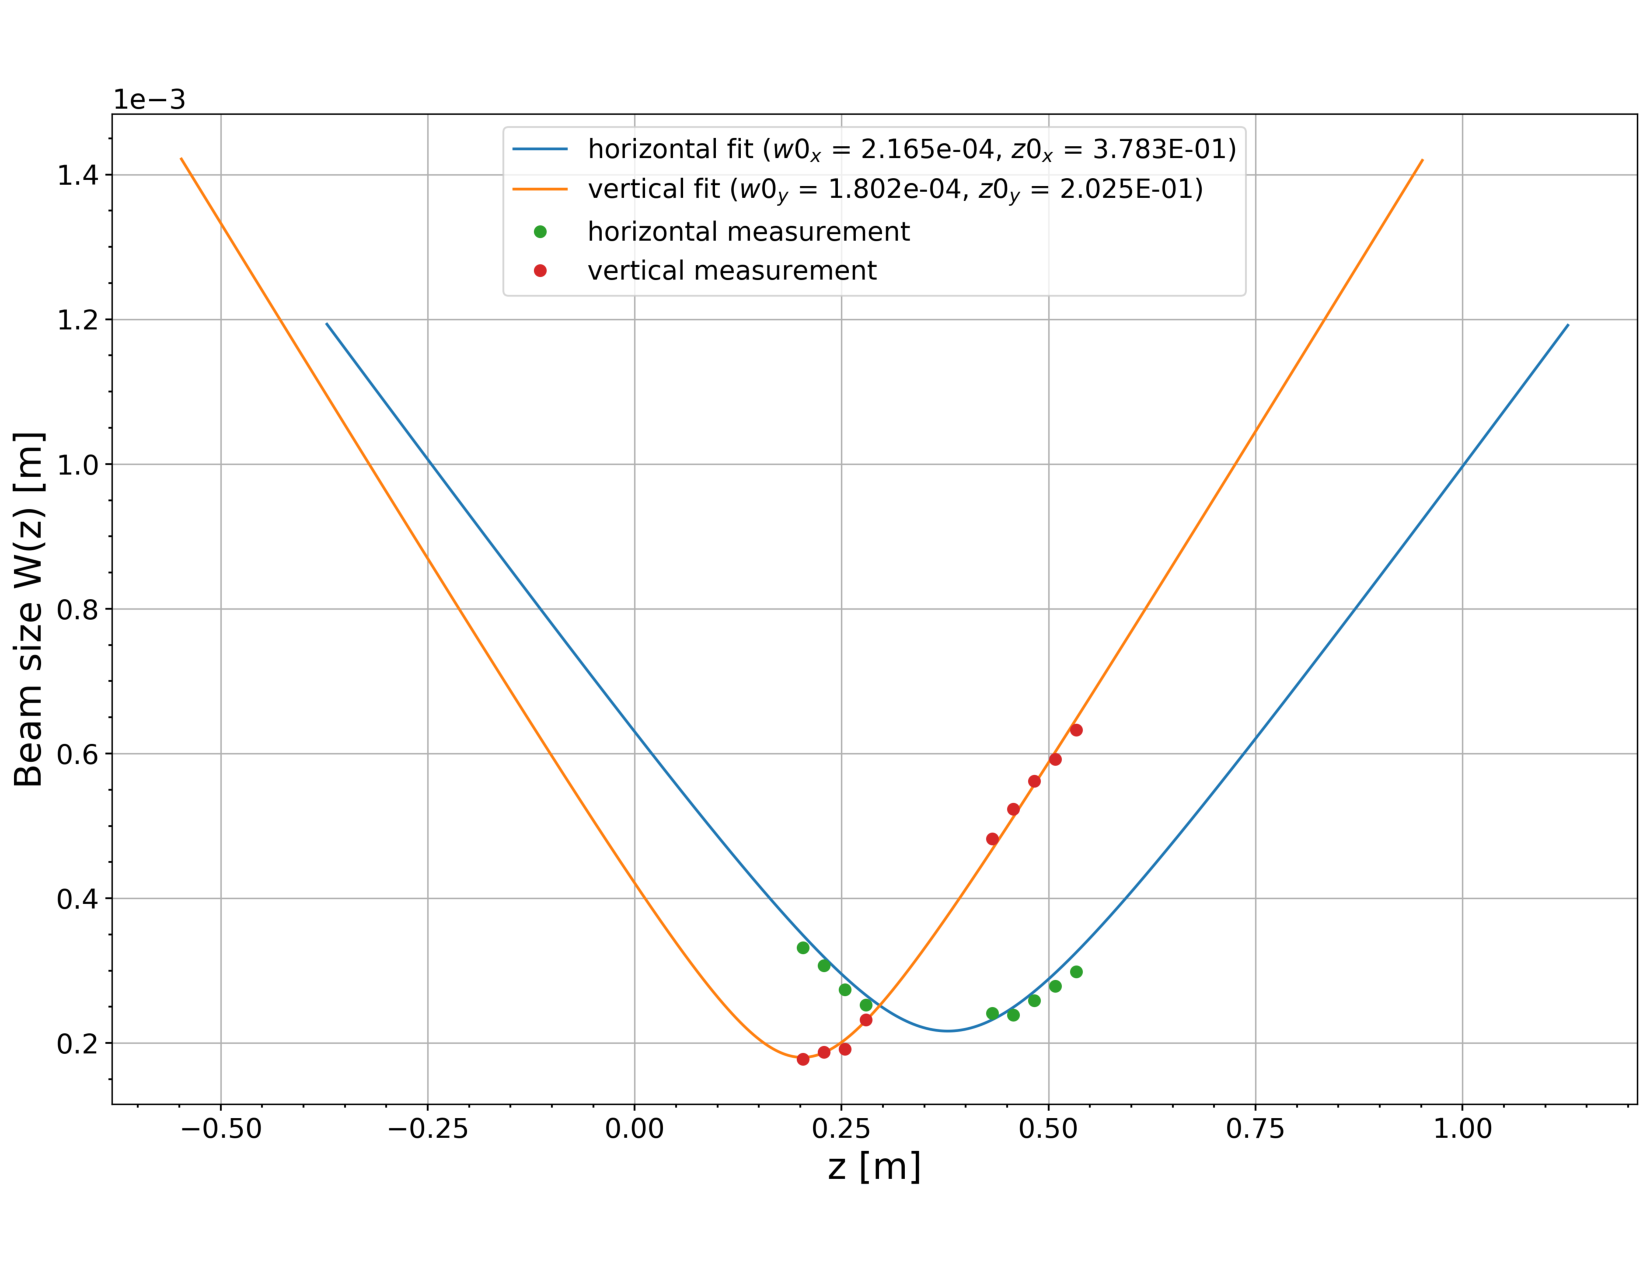
\includegraphics[width=\textwidth]{figs/ALGAAS/beam_scans/12_18_2020_preMMT.pdf}
\caption{Beam scan taken from SM5 (Steering mirror 5)}
\label{fig:beamscan2020}
\end{figure}


\subsection{``Just another mode matching tool" (JAMMT) solution}
\subsection{Post MMT beam scan}

\begin{figure}[H]
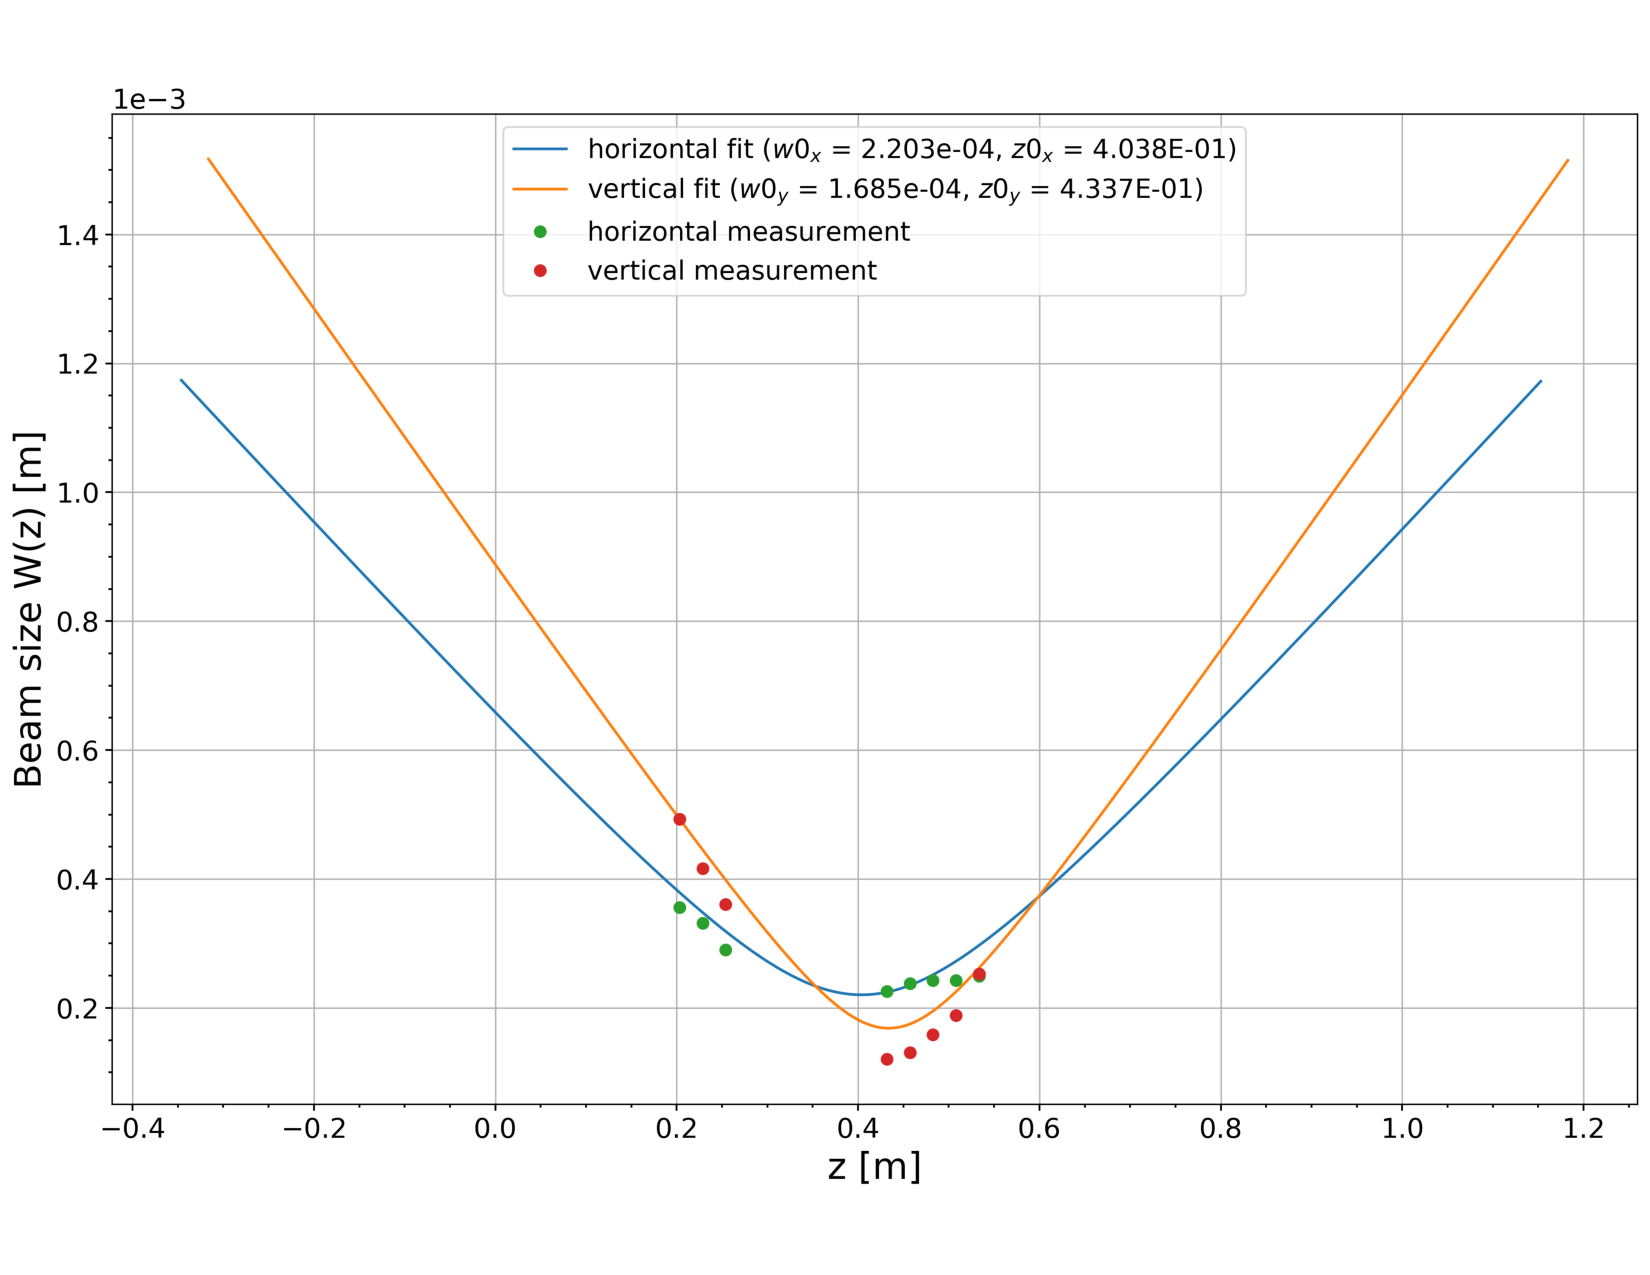
\includegraphics[width=\textwidth]{figs/ALGAAS/beam_scans/01_12_2021_postMMT.pdf}
\caption{Beam scan taken from SM6. Sampling points before SM7 and after the first cavity iris.}
\label{fig:beamscan2021}
\end{figure}

\subsection{Laser PZT sweep}

\begin{figure}[H]
	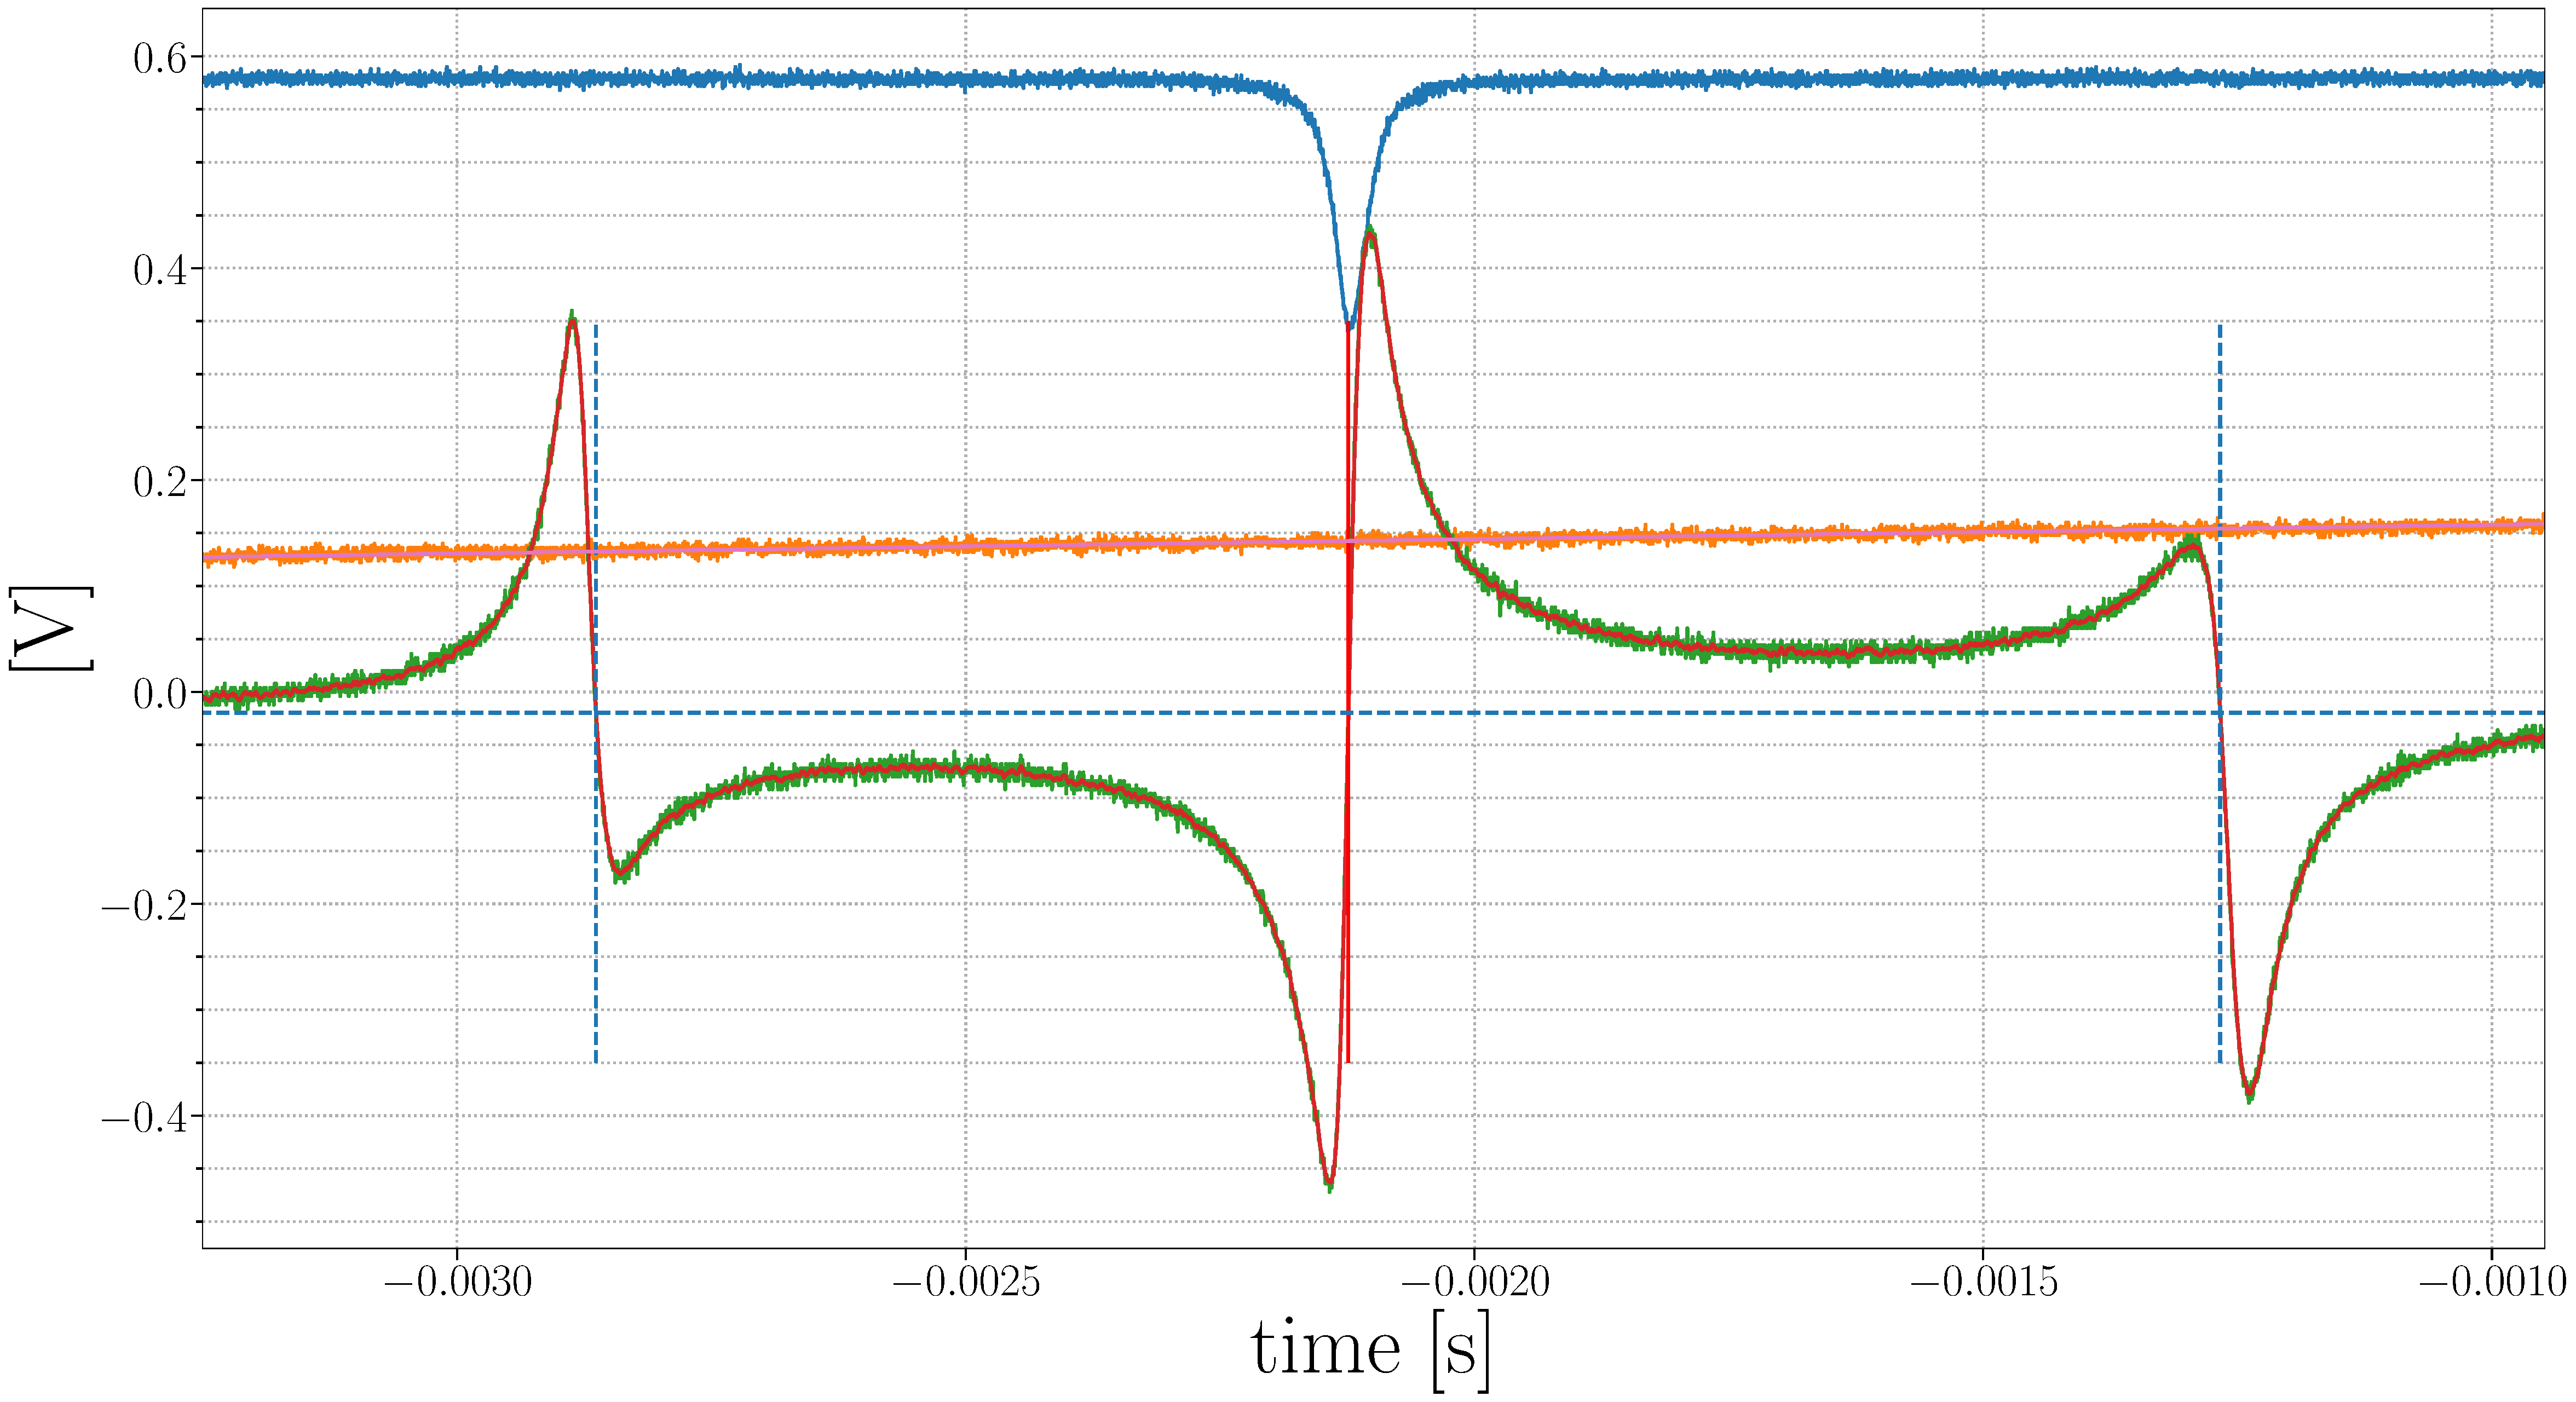
\includegraphics[width=\textwidth]{figs/ALGAAS/pdh_measured.pdf}
	\caption{Ramping voltage sent to the laser PZT while probing the mixer output. The sweep was performed for sample cavity of length notes}
\label{fig:pdhmeasured}
\end{figure}

\newpage

\section{Assembly blueprints and alternative views}

\subsection{Assembly 1}

\subsubsection{Cross section}

\subsubsection{Electrodes}

\subsubsection{Iteration 1.1}

\begin{figure}[!ht]
	\begin{subcaptiongroup}
		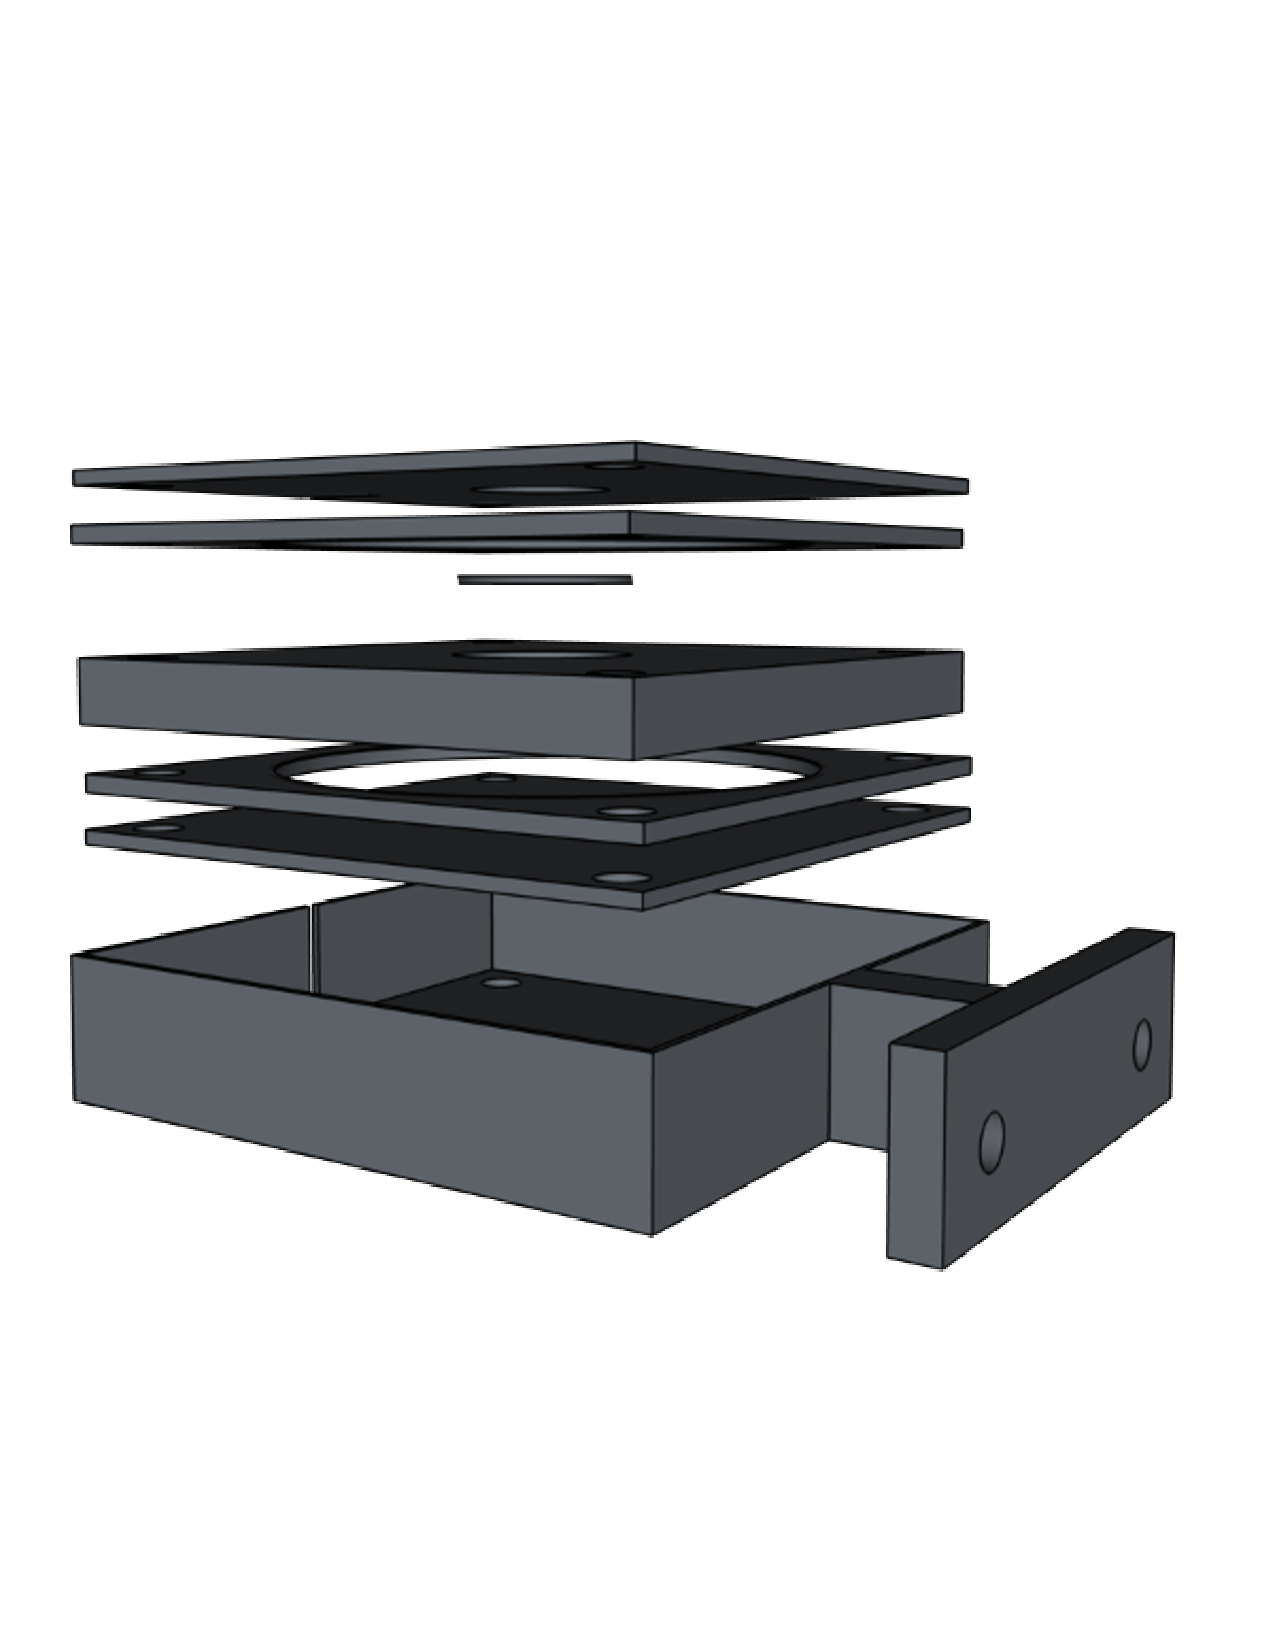
\includegraphics[width=.5\textwidth]{figs/ALGAAS/assemblies/assembly0/assembly0.pdf}
		\phantomcaption\label{A0}
		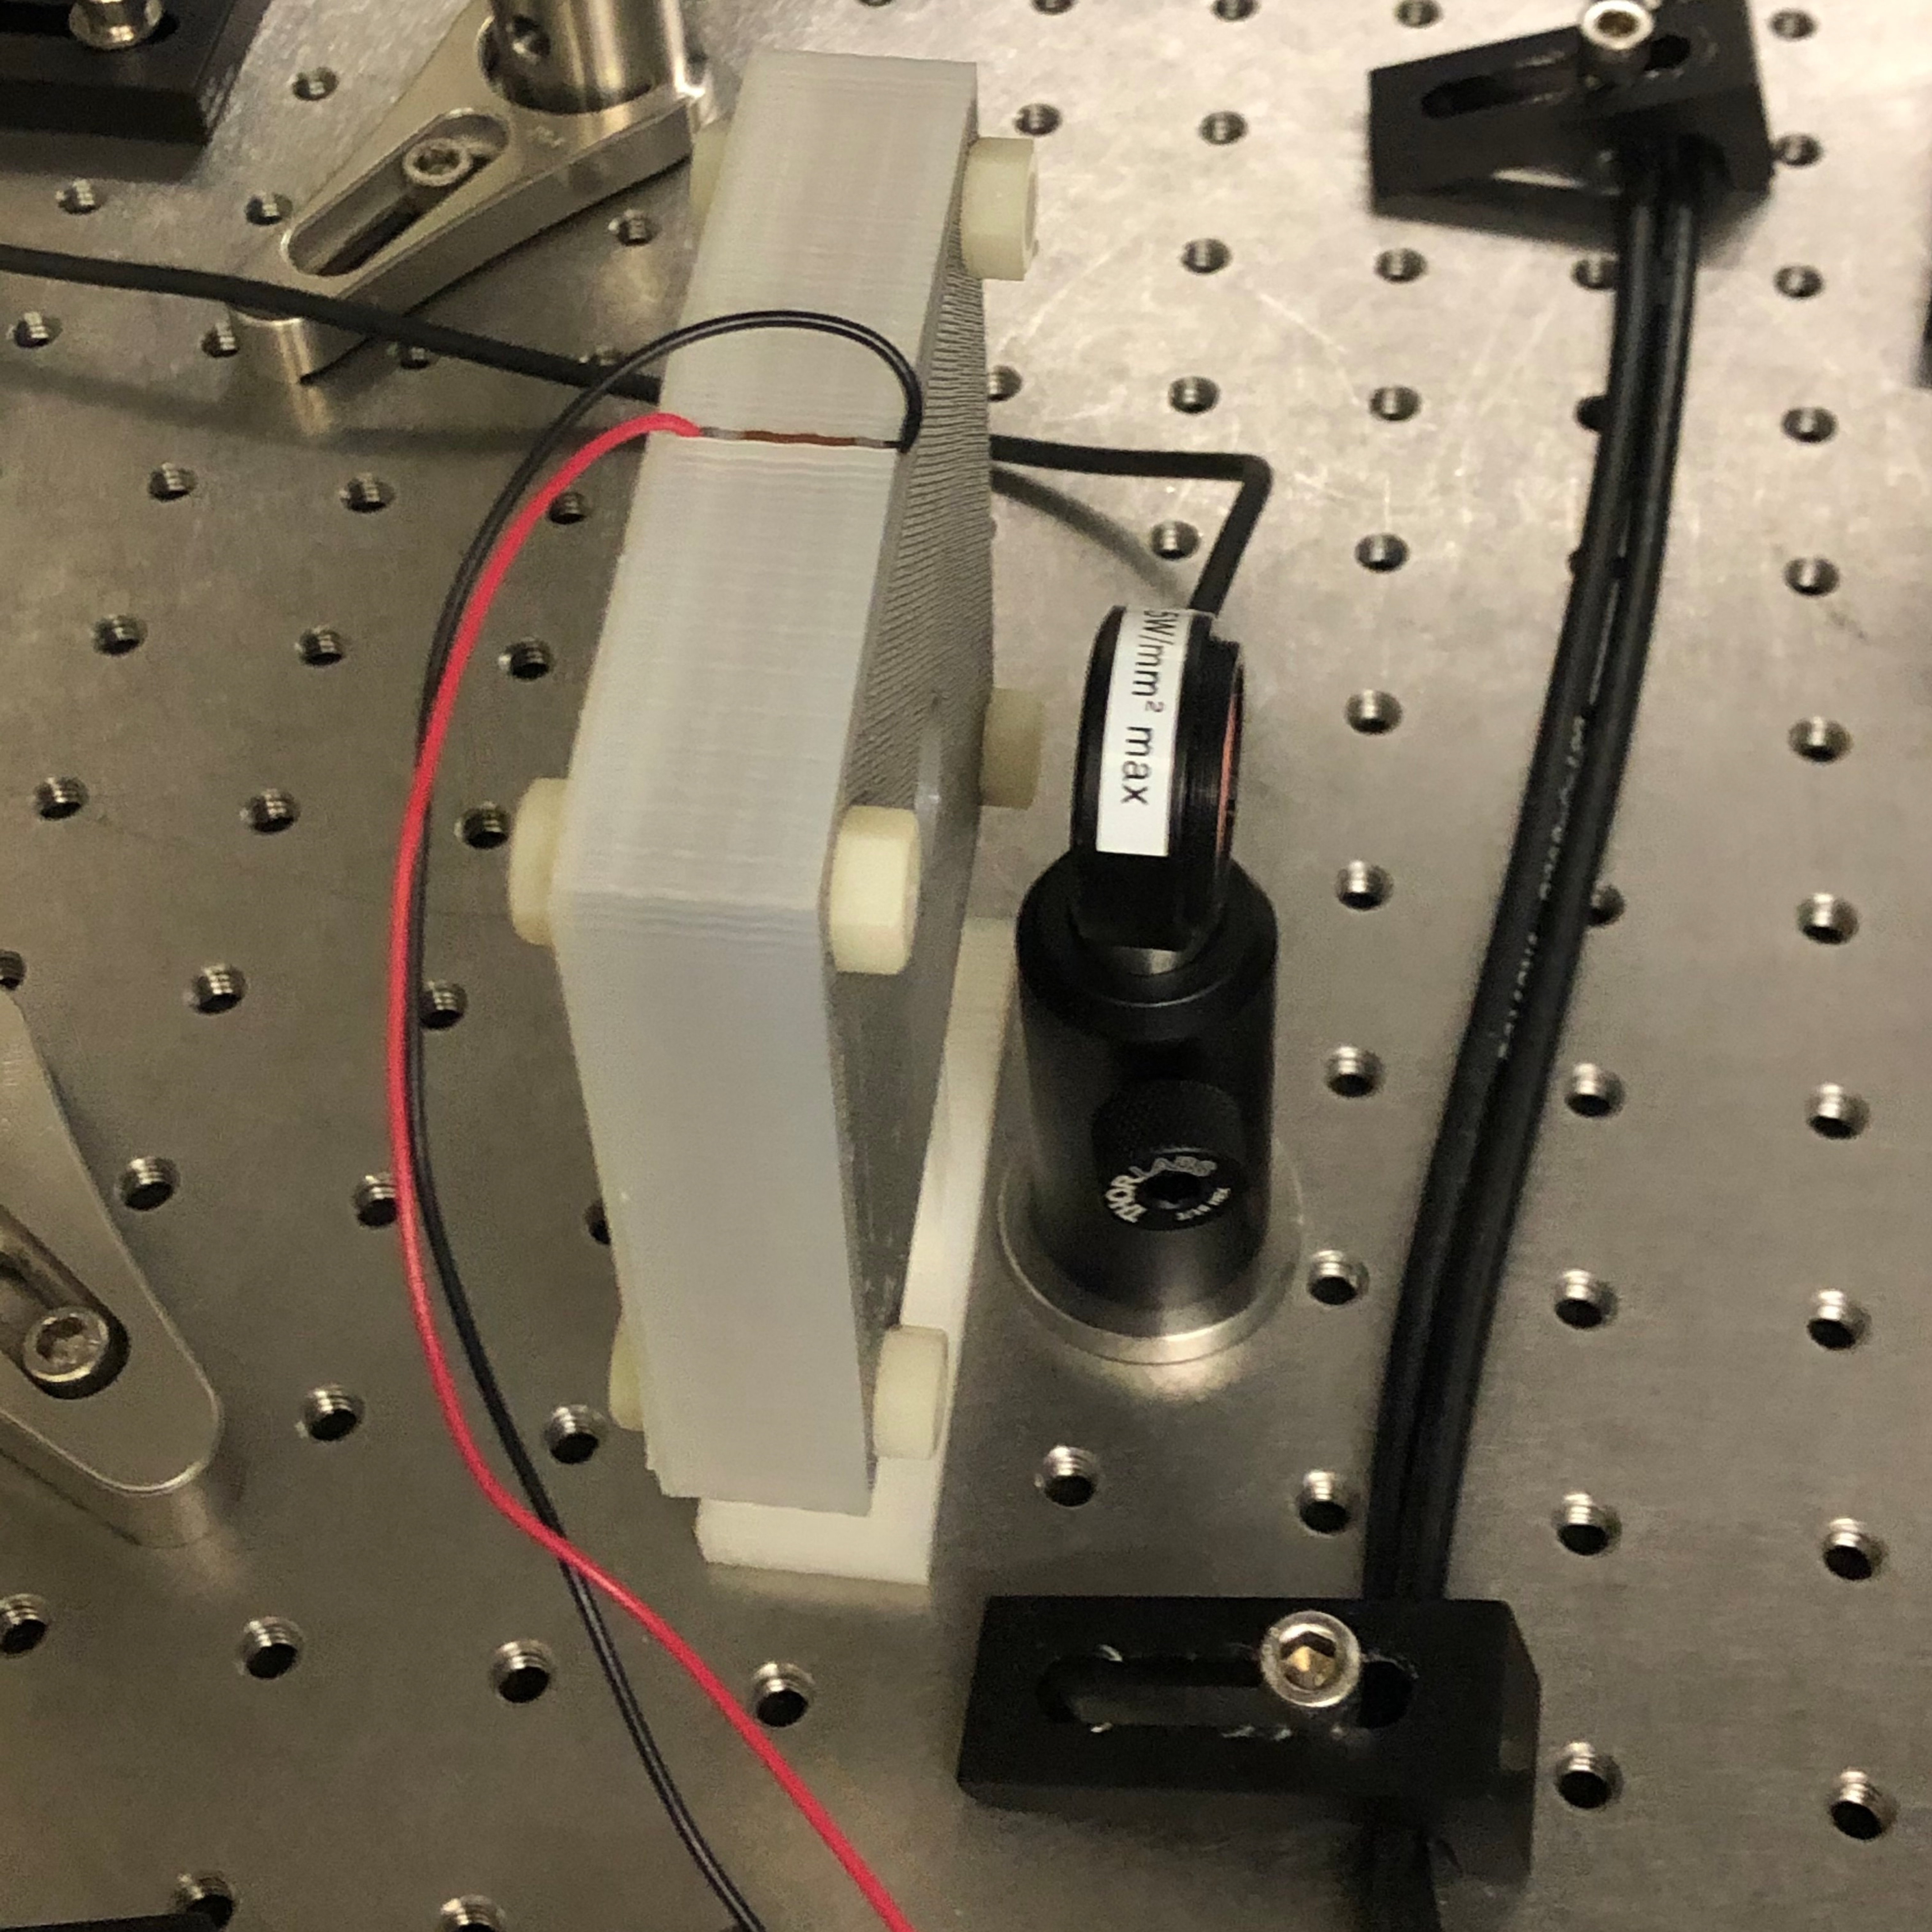
\includegraphics[width=.5\textwidth]{figs/ALGAAS/assemblies/assembly0/assembly0_incident_power.pdf}
 		\phantomcaption\label{A0inc}
	\end{subcaptiongroup}
  \caption{Assembly 0 was constructed to meet the criteria of providing a non-conductive housing for the electrode / sample assembly while maintaining a fixed length spacing using parts 3d printed with polylactic acid (PLA).}
  \label{fig:assembly0bp}
\end{figure}
\FloatBarrier

\subsubsection{Iteration 1.2}
\begin{figure}[!ht]
	\begin{subcaptiongroup}
		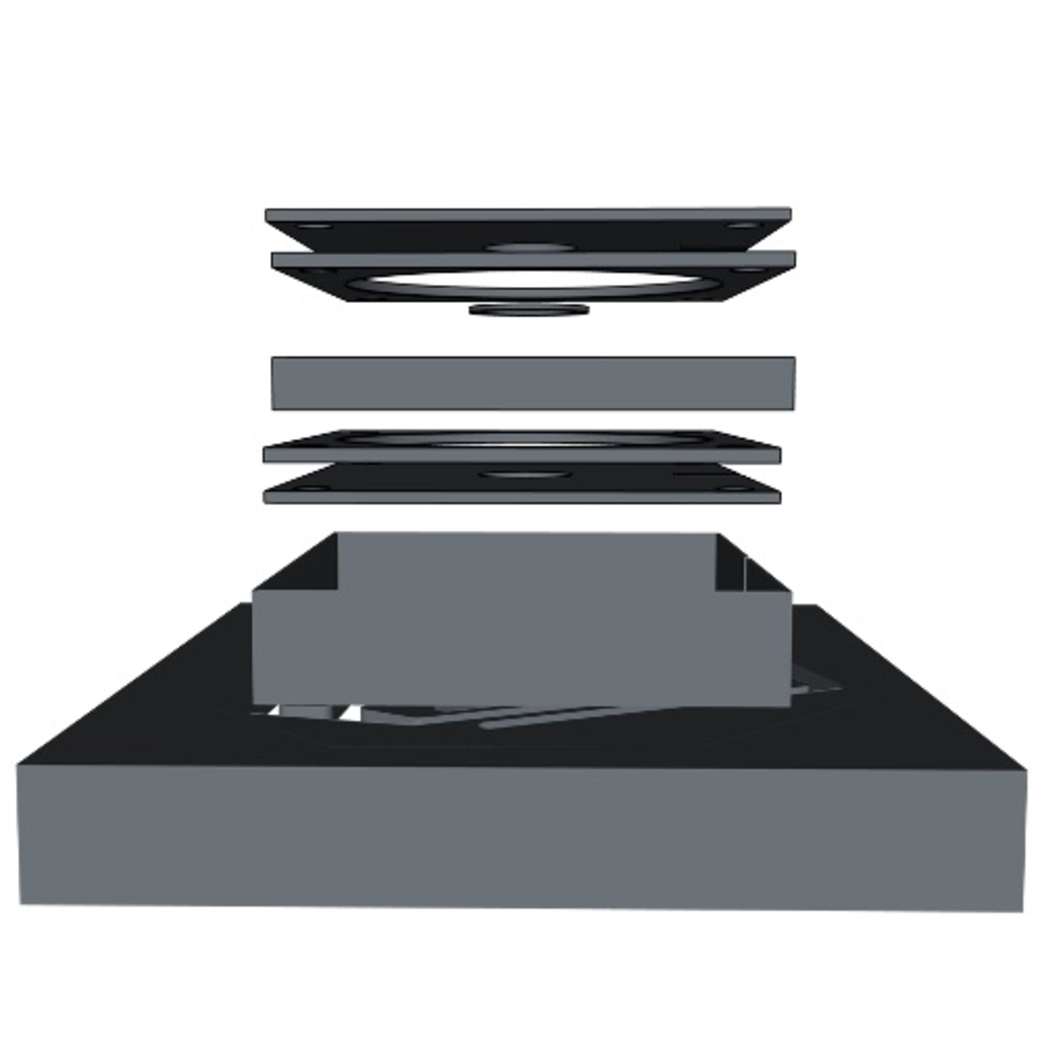
\includegraphics[width=.5\textwidth]{figs/ALGAAS/assemblies/assembly1/assembly1_dissassembled.pdf}
		\phantomcaption\label{A1pt2CAD}
		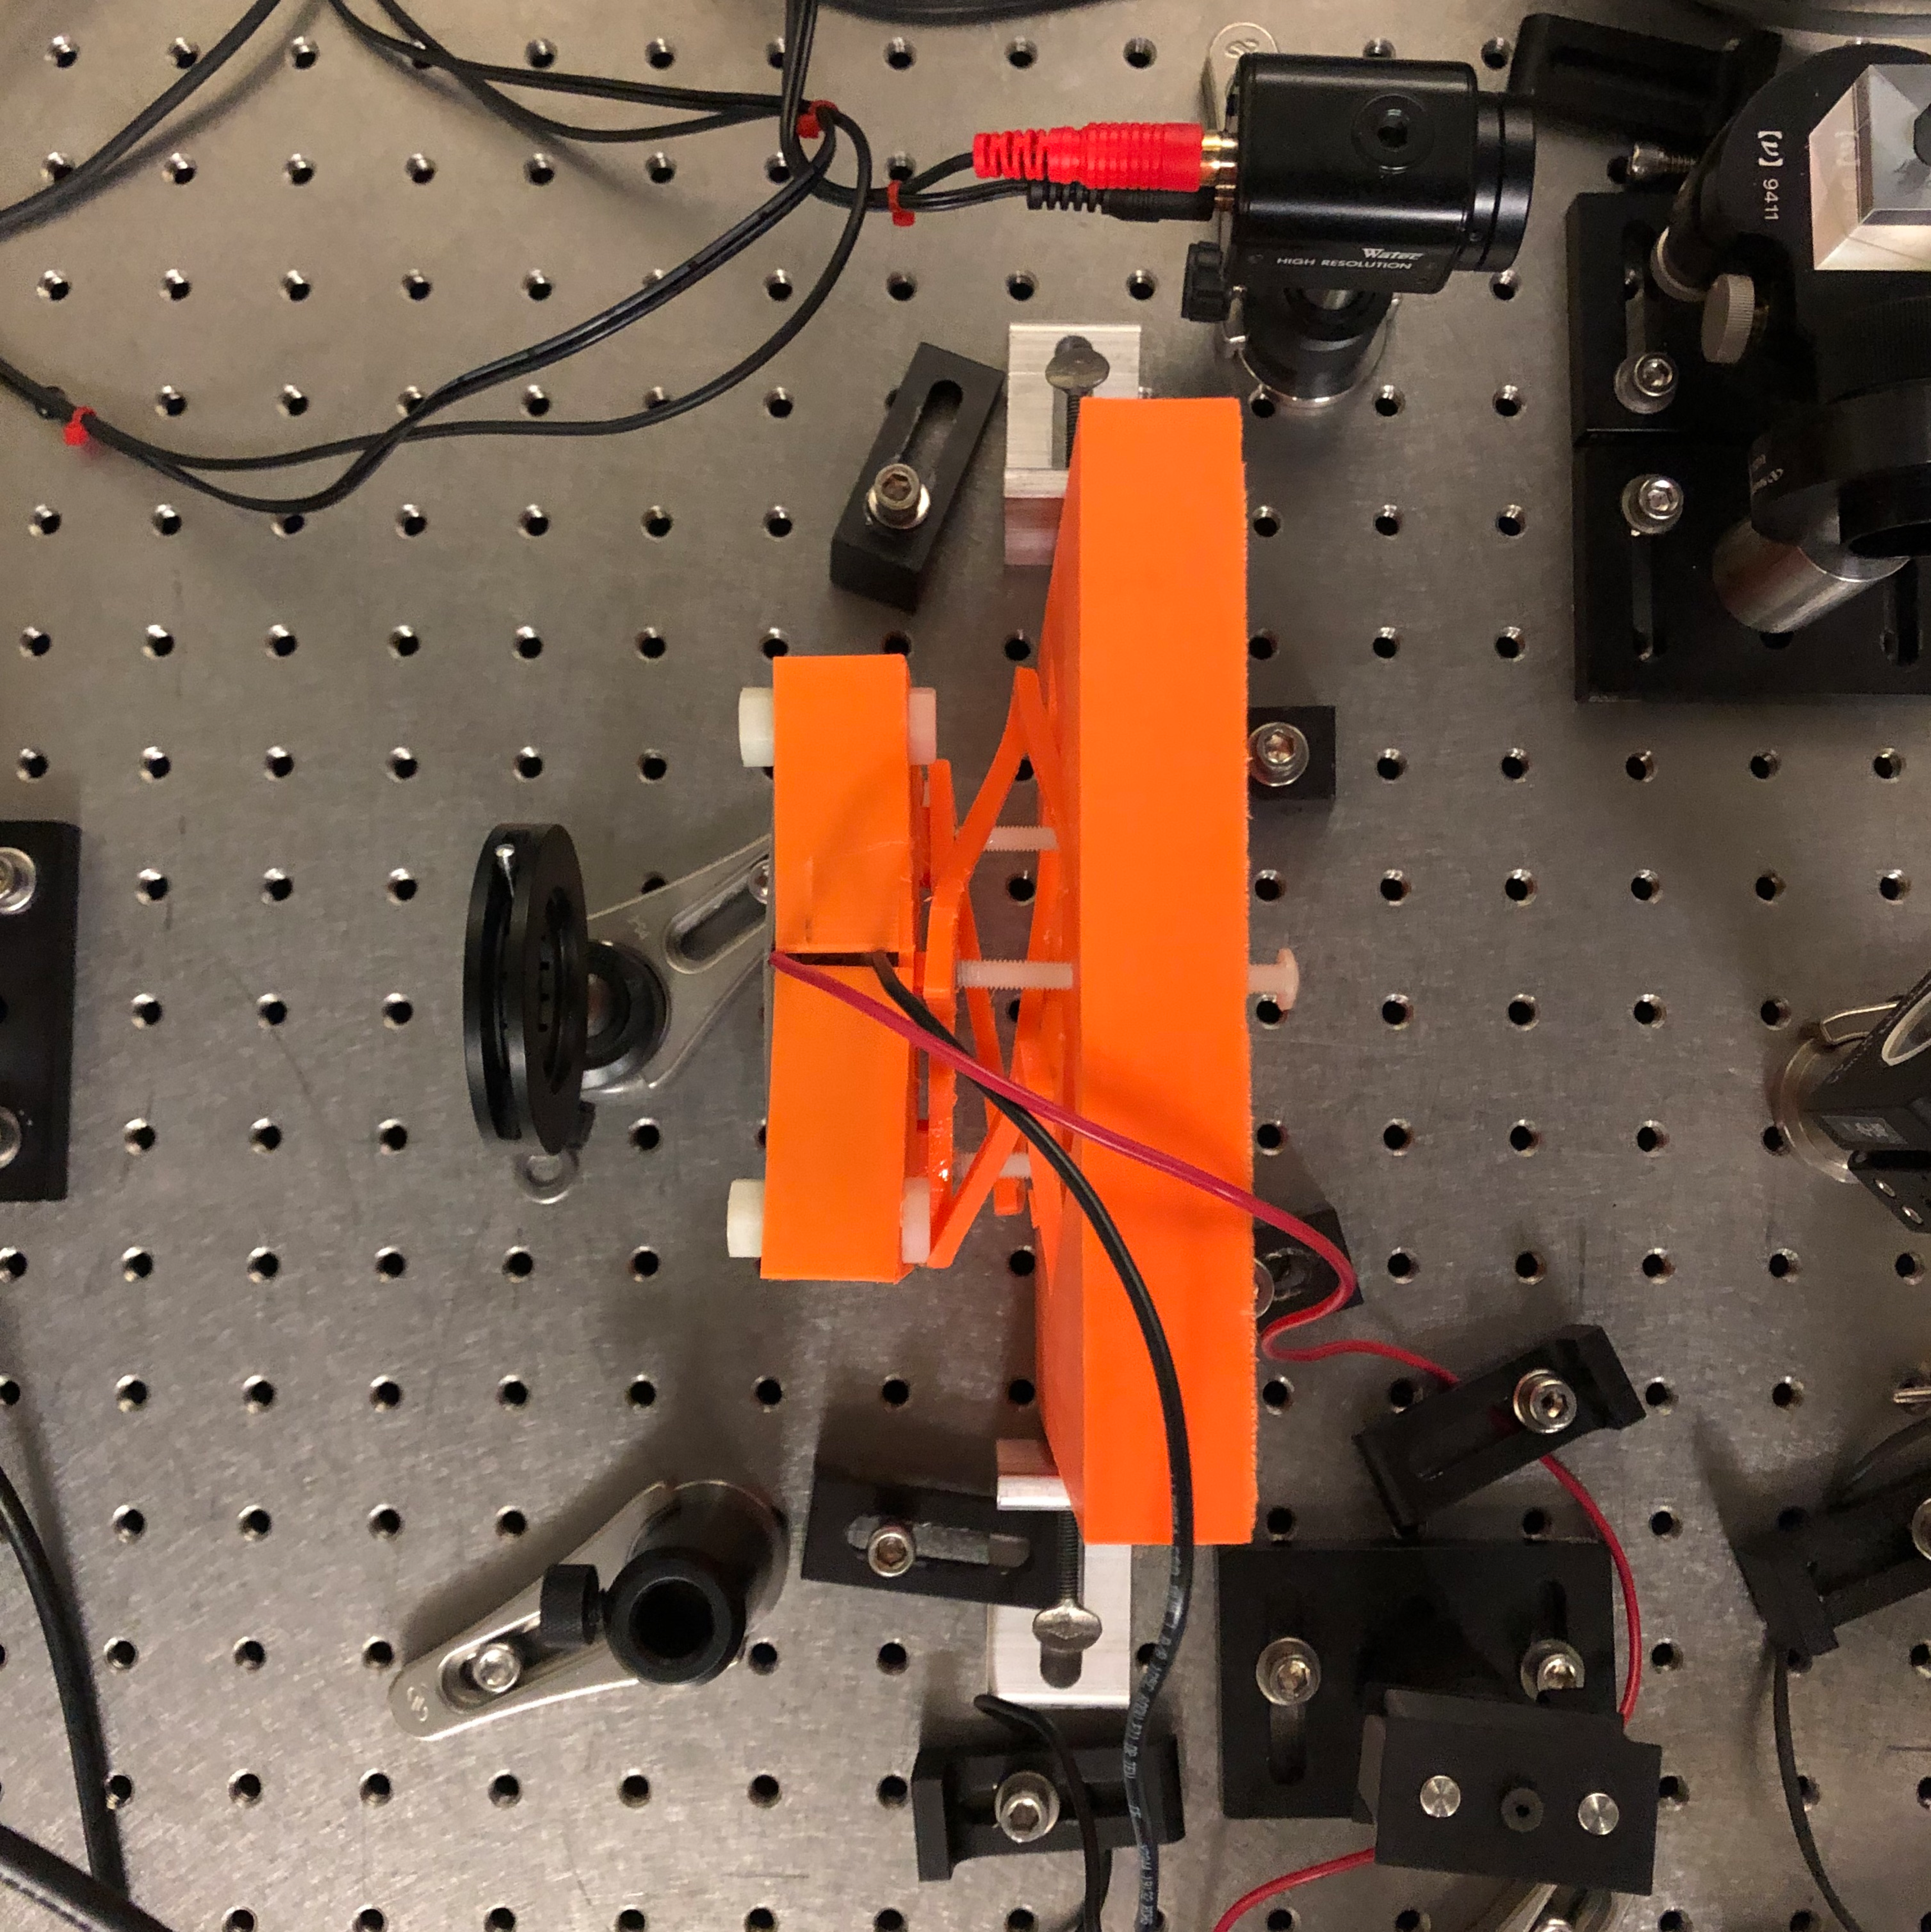
\includegraphics[width=.5\textwidth]{figs/ALGAAS/assemblies/assembly1/assembly1_insitu2.pdf}
		\phantomcaption\label{A1pt2pic}	
	\end{subcaptiongroup}
	\caption{Assembly 1 was constructed to meet the criteria of providing a non-conductive housing for the electrode / sample assembly while maintaining a fixed length spacing using parts 3d printed with polylactic acid (PLA).}
	\label{fig:assembly1bp}
\end{figure}
\FloatBarrier

\subsubsection{Iteration 1.3}
\begin{figure}[!ht]
	\begin{subcaptiongroup}
		\includegraphics[width=.5\textwidth]{figs/ALGAAS/assemblies/assembly1/assembly1_mod_front.pdf}
		\phantomcaption\label{A1pt3CAD}
		\includegraphics[width=.5\textwidth]{figs/ALGAAS/assemblies/assembly1/assembly1_mod_side.pdf}
		\phantomcaption\label{A1pt3pic}
	\end{subcaptiongroup}
	\caption{A modification implemented with the intention of reducing pitch dithering while still having control of DC YAW}
	\label{fig:assembly1mod}
\end{figure}

\newpage

\subsection{Assembly 2}
\subsubsection{Cross section}

\subsubsection{Electrodes}

\begin{figure}[H]
  \centering
  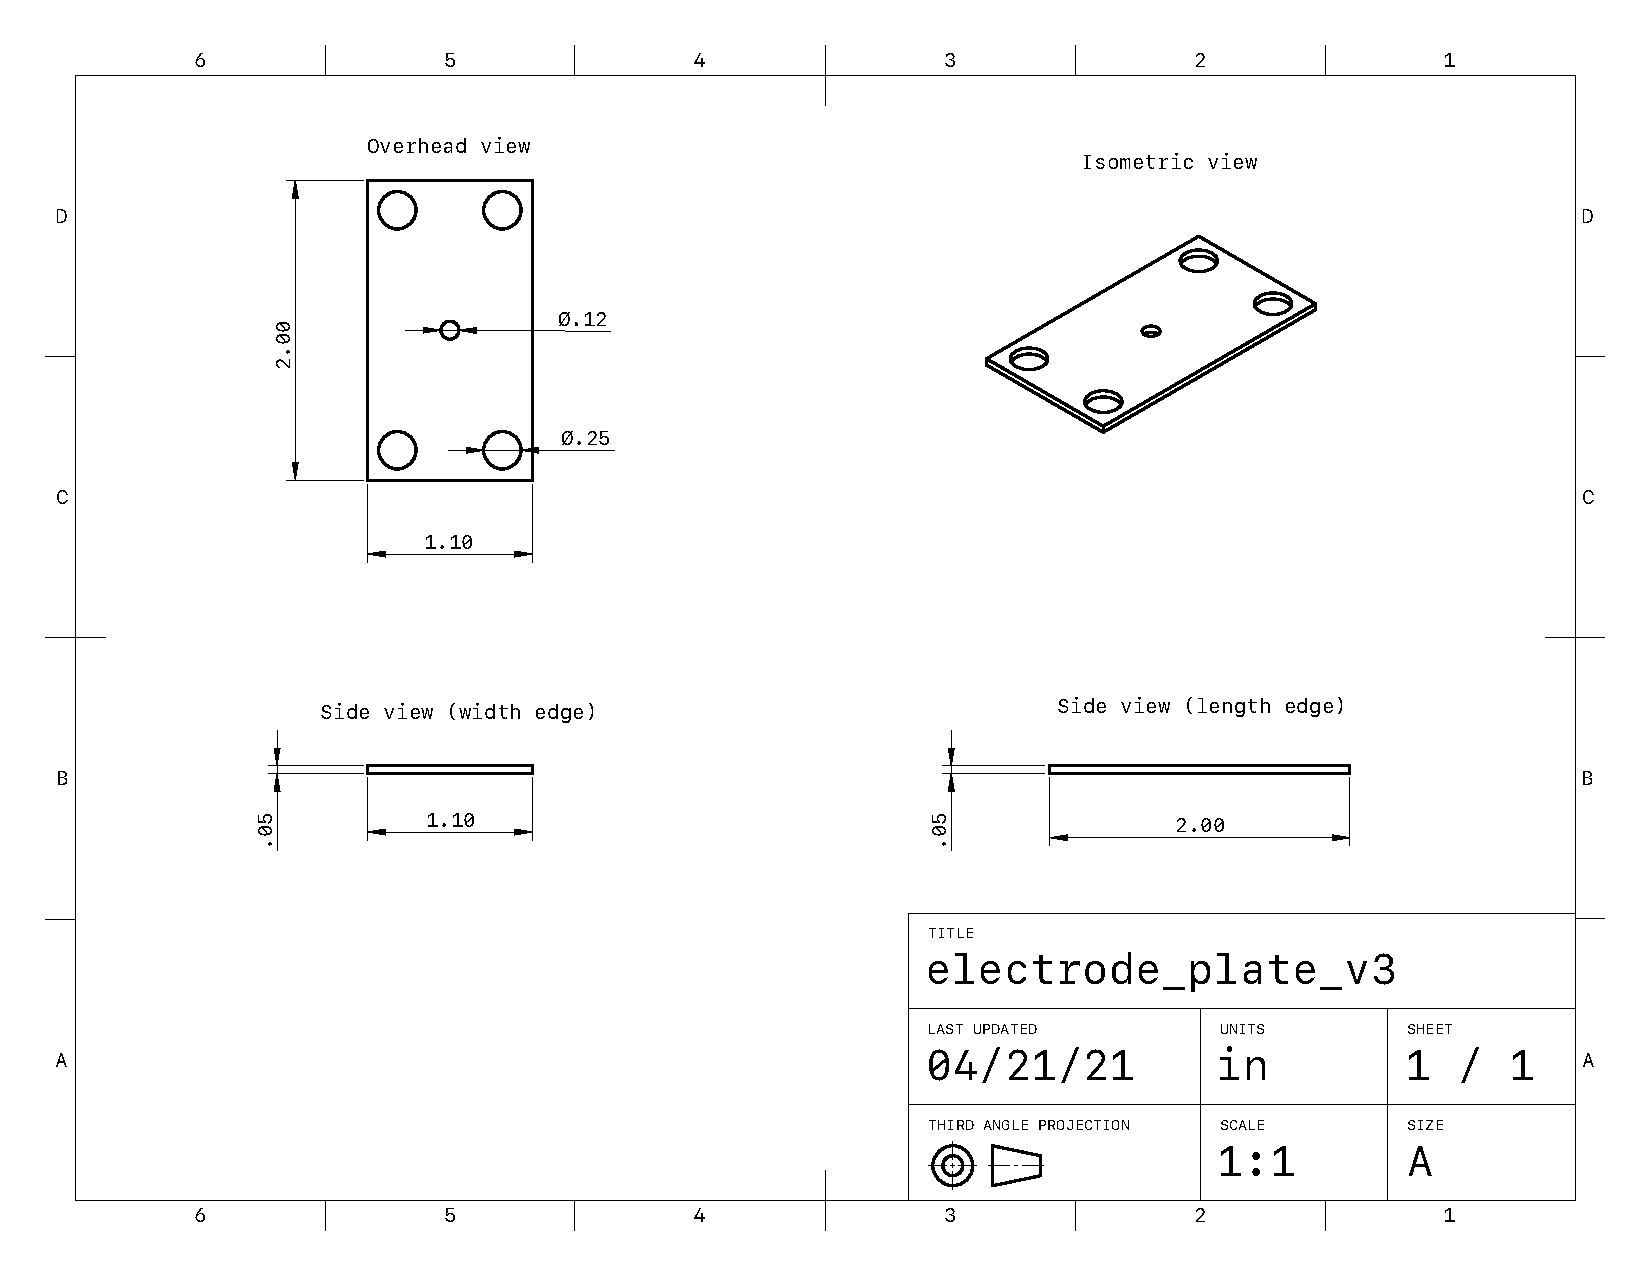
\includegraphics[width=.776\textwidth]{figs/ALGAAS/assemblies/assembly2/assembly2_electrode.pdf}
  \caption{Rectangular (.05"X1.1"X2") plates made of aluminum.}
\end{figure}

\newpage
\subsubsection{Iteration 2.1}
\begin{figure}[!ht]
	\centering
	\begin{subcaptiongroup}
		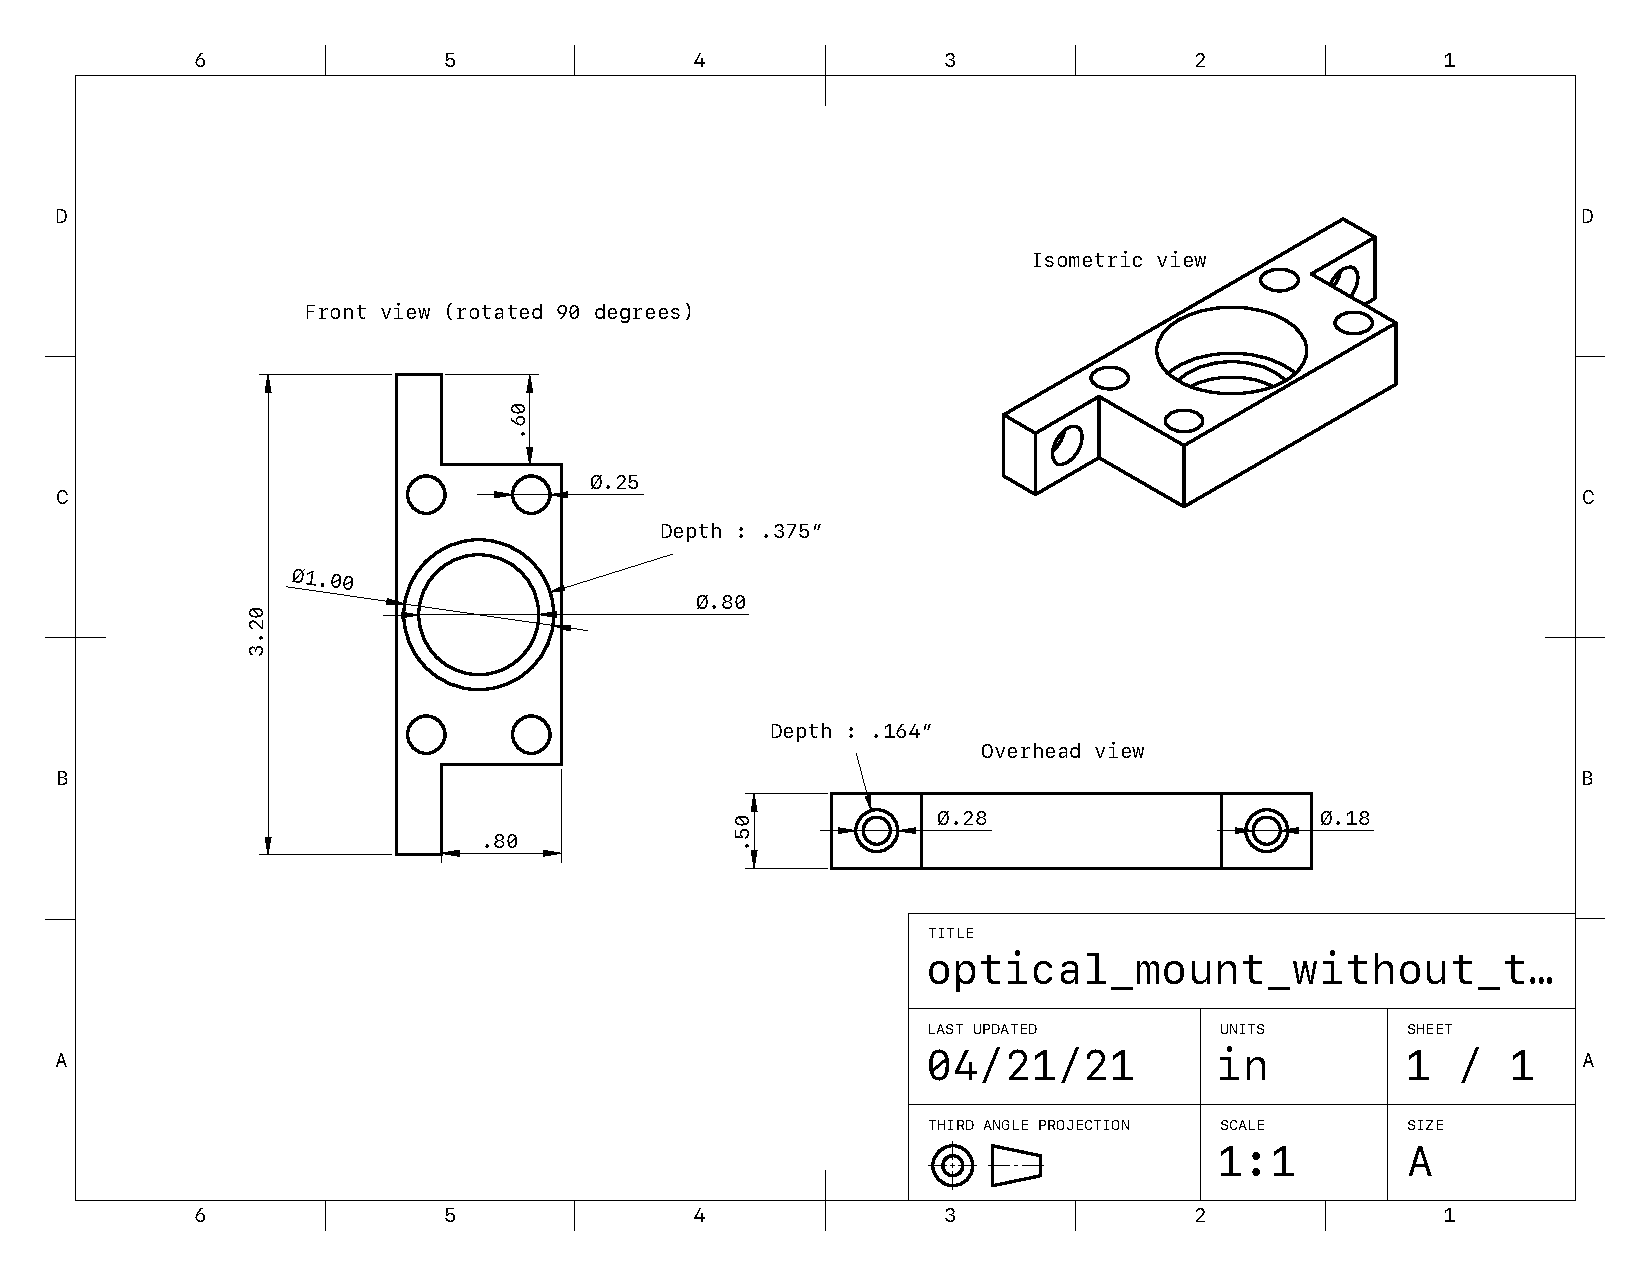
\includegraphics[width=.76\textwidth]{figs/ALGAAS/assemblies/assembly2/assembly2_PVC_mount.pdf}
		\phantomcaption\label{A2PVCmount}
		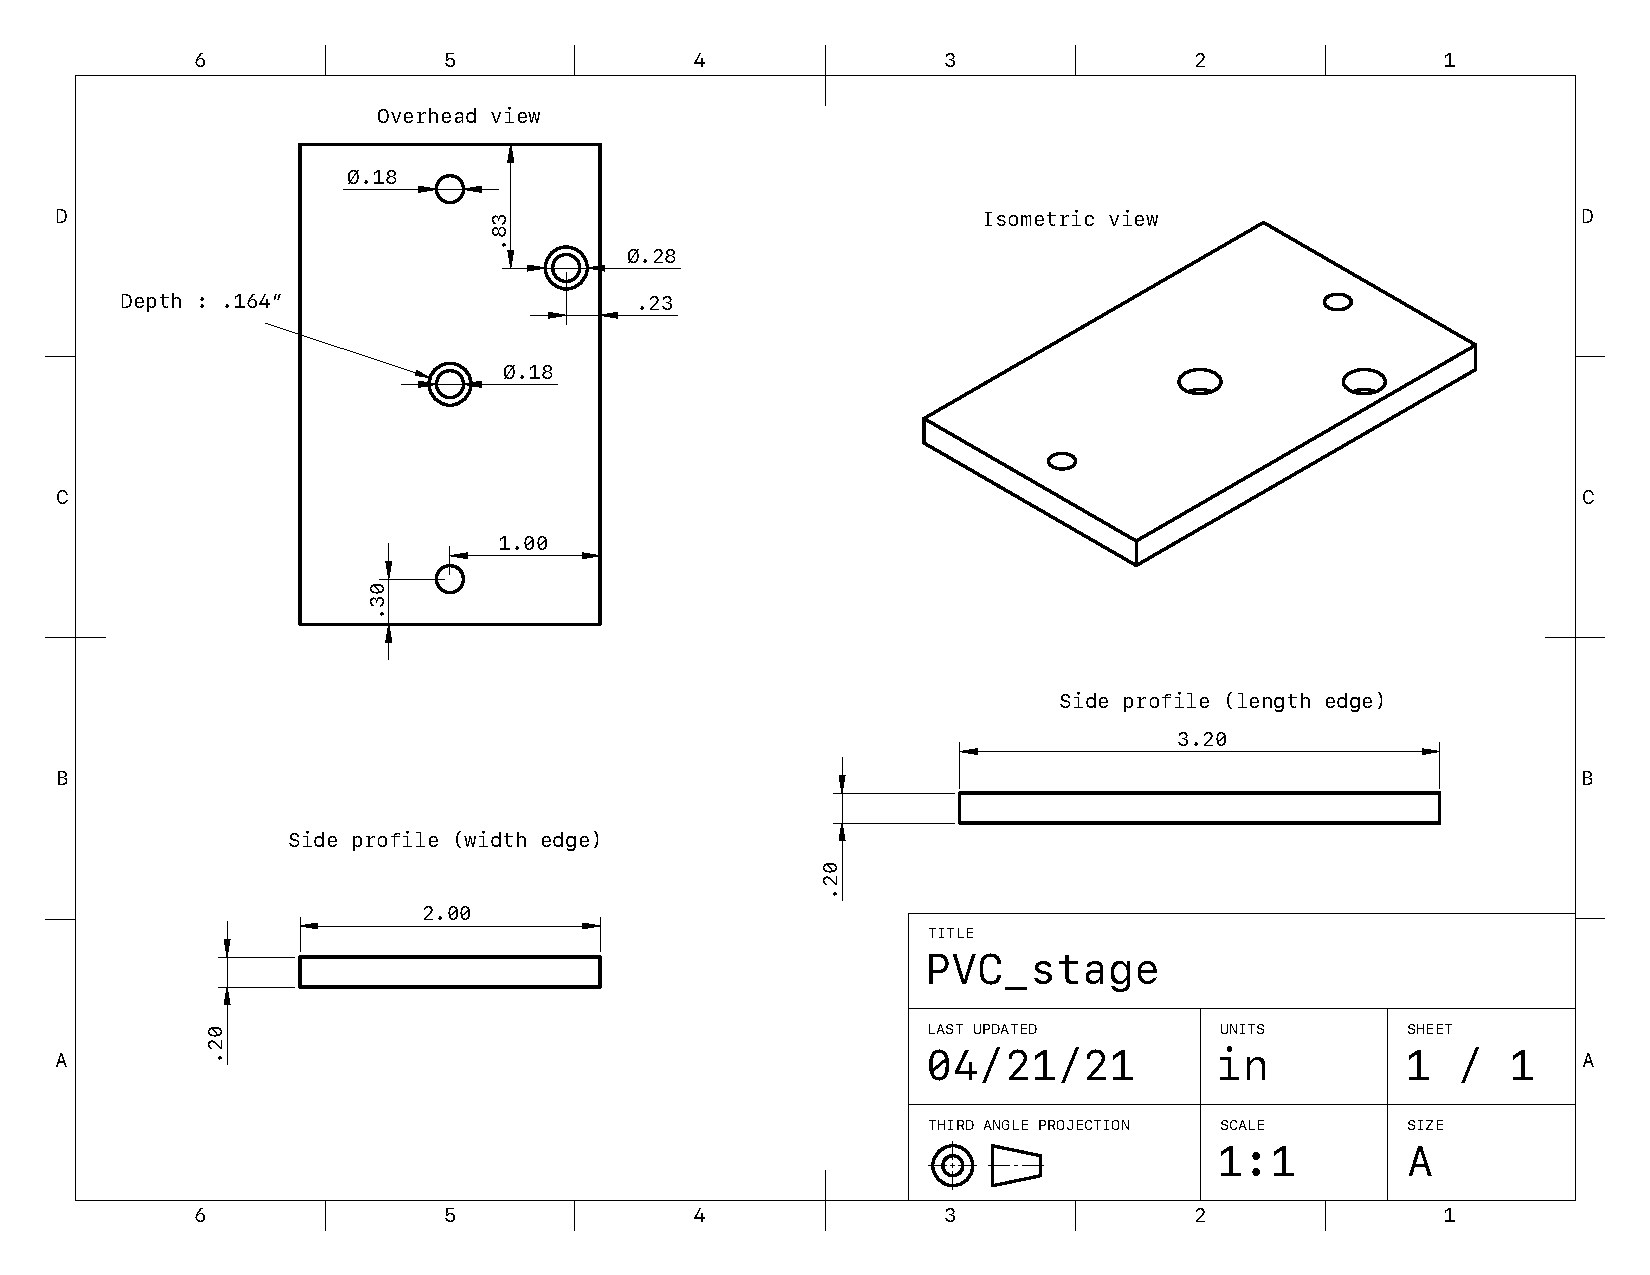
\includegraphics[width=.76\textwidth]{figs/ALGAAS/assemblies/assembly2/assembly2_PVC_stage.pdf}
		\phantomcaption\label{A2PVCstage}
	\end{subcaptiongroup}
	\caption{A design iteration of the assembly 2 mounts. Materials tried varied from PVC, PLA, and PETG. Quarter inch holes are bored in order to pass nylon screws holding electrode plates fixed to the mount.}
	\label{fig:assembly2bp}
\end{figure}
\FloatBarrier

\subsubsection{Iteration 2.2}

\subsubsection{3D printed w/ MACOR spacers}

\textcolor{red}{Insert blueprints}

\textcolor{red}{Insert printed results}

\newpage

\section{Assembly 3 [MACOR] (blueprint)}
\subsubsection{Cross section}
\subsubsection{Electrodes}

\subsubsection{Iteration 3.0}
\begin{figure}[H]
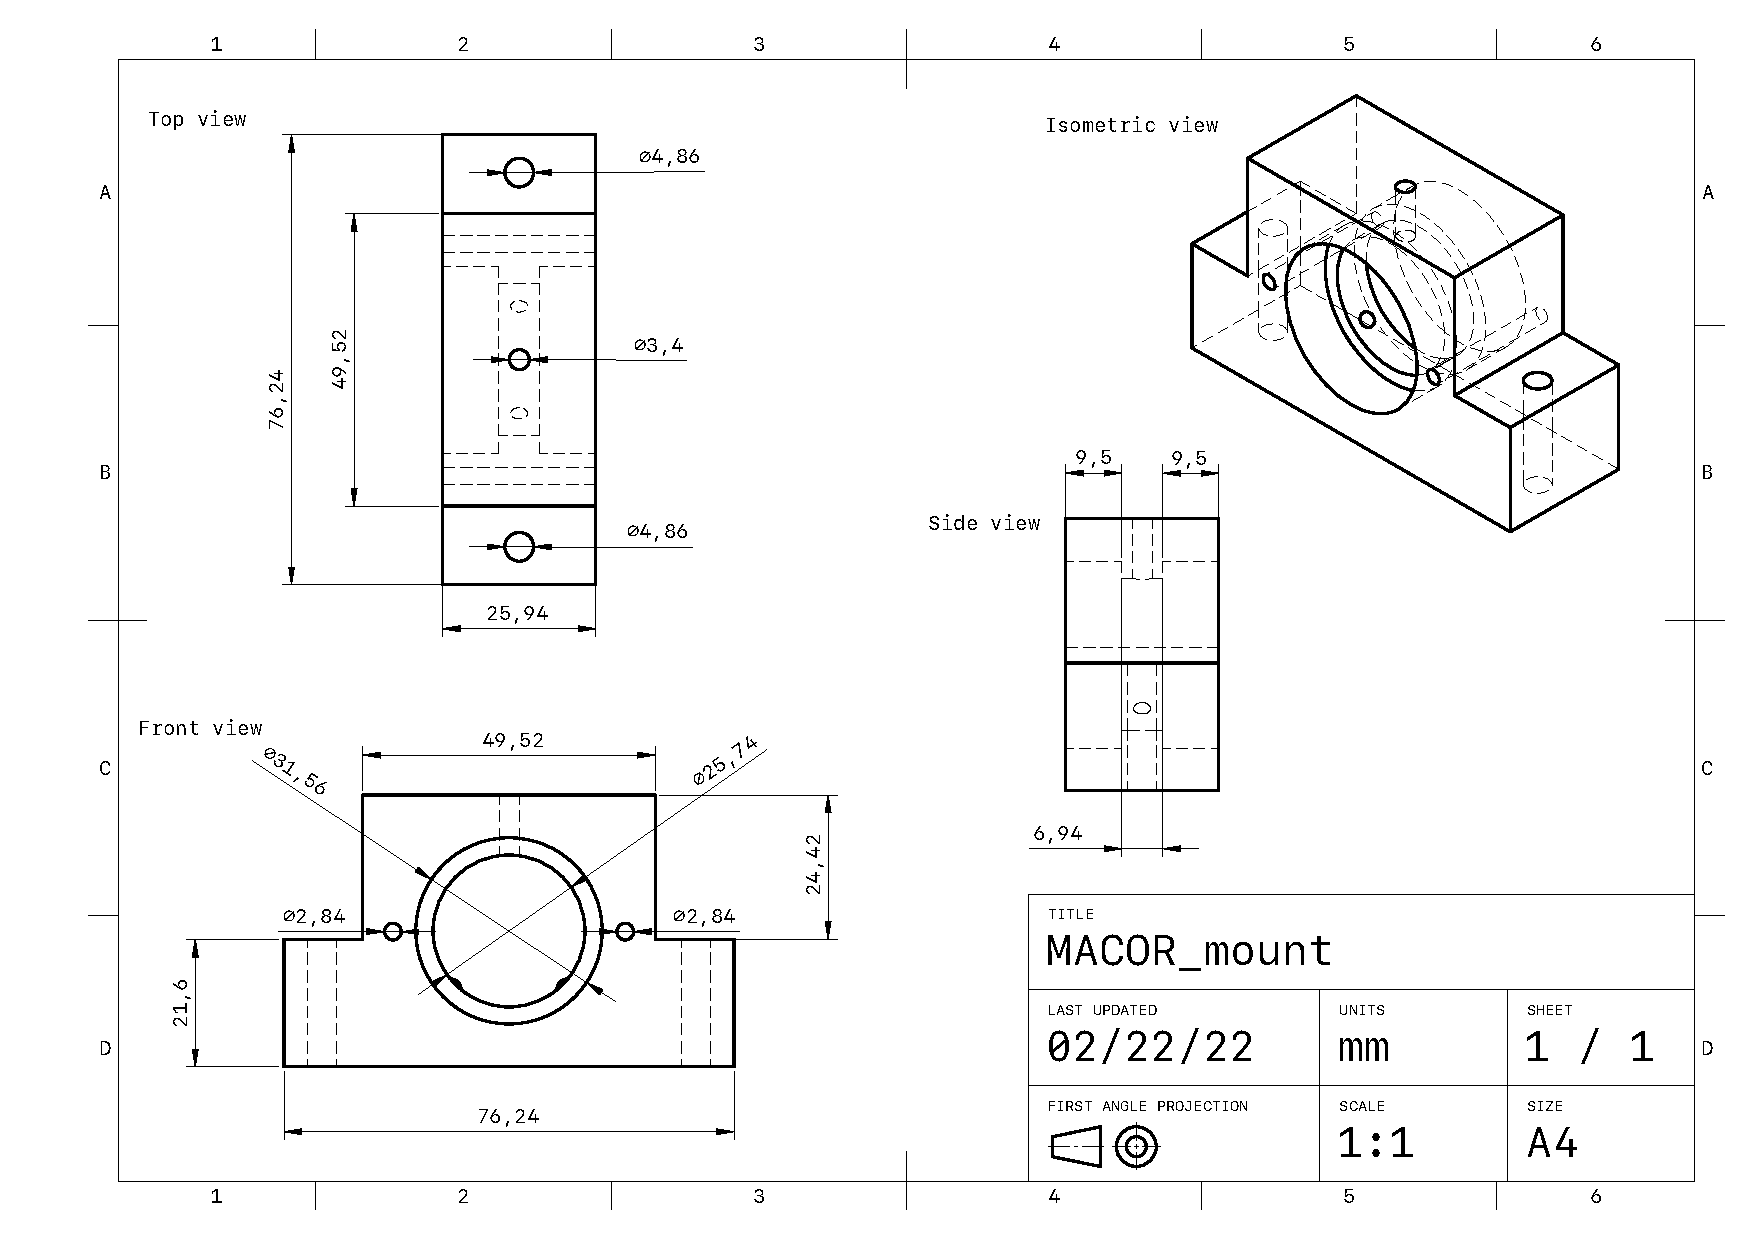
\includegraphics[width=\textwidth]{figs/ALGAAS/assemblies/assembly3/MACOR_mount.pdf}
\caption{MACOR mount design constucted in Shapr3D}
\label{fig:macormountdesign}
\end{figure}

\mbox{}
\vfill

\section{Calibration}\label{sec:calibration}
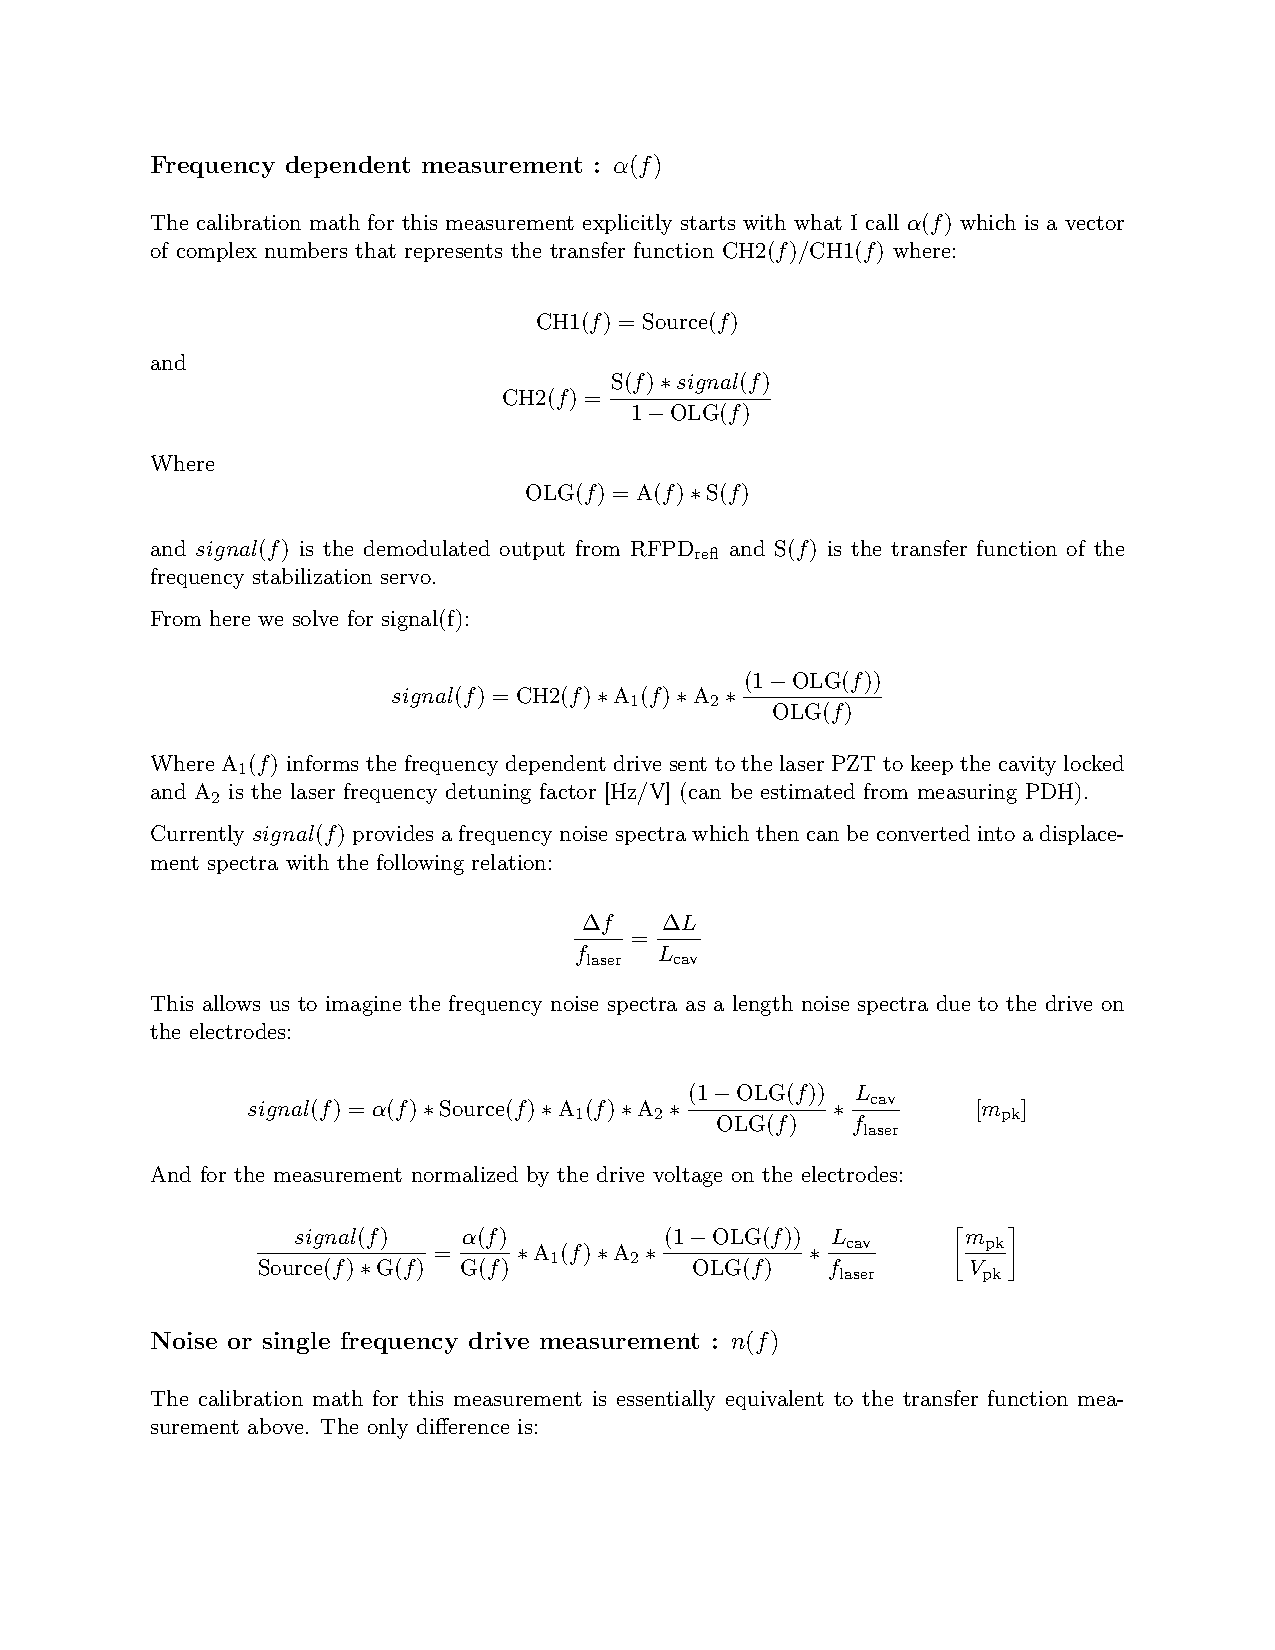
\includepdf[pages=-, pagecommand={}]{notes/pockels_calibration.pdf}

\section{Single frequency}

\section{Laplace calculator / code}

\textcolor{red}{Snippets of explicit code with a block diagram for clarity}

\section{HVA}

\section{FSS}

\begin{figure}[H]
  \begin{center}
    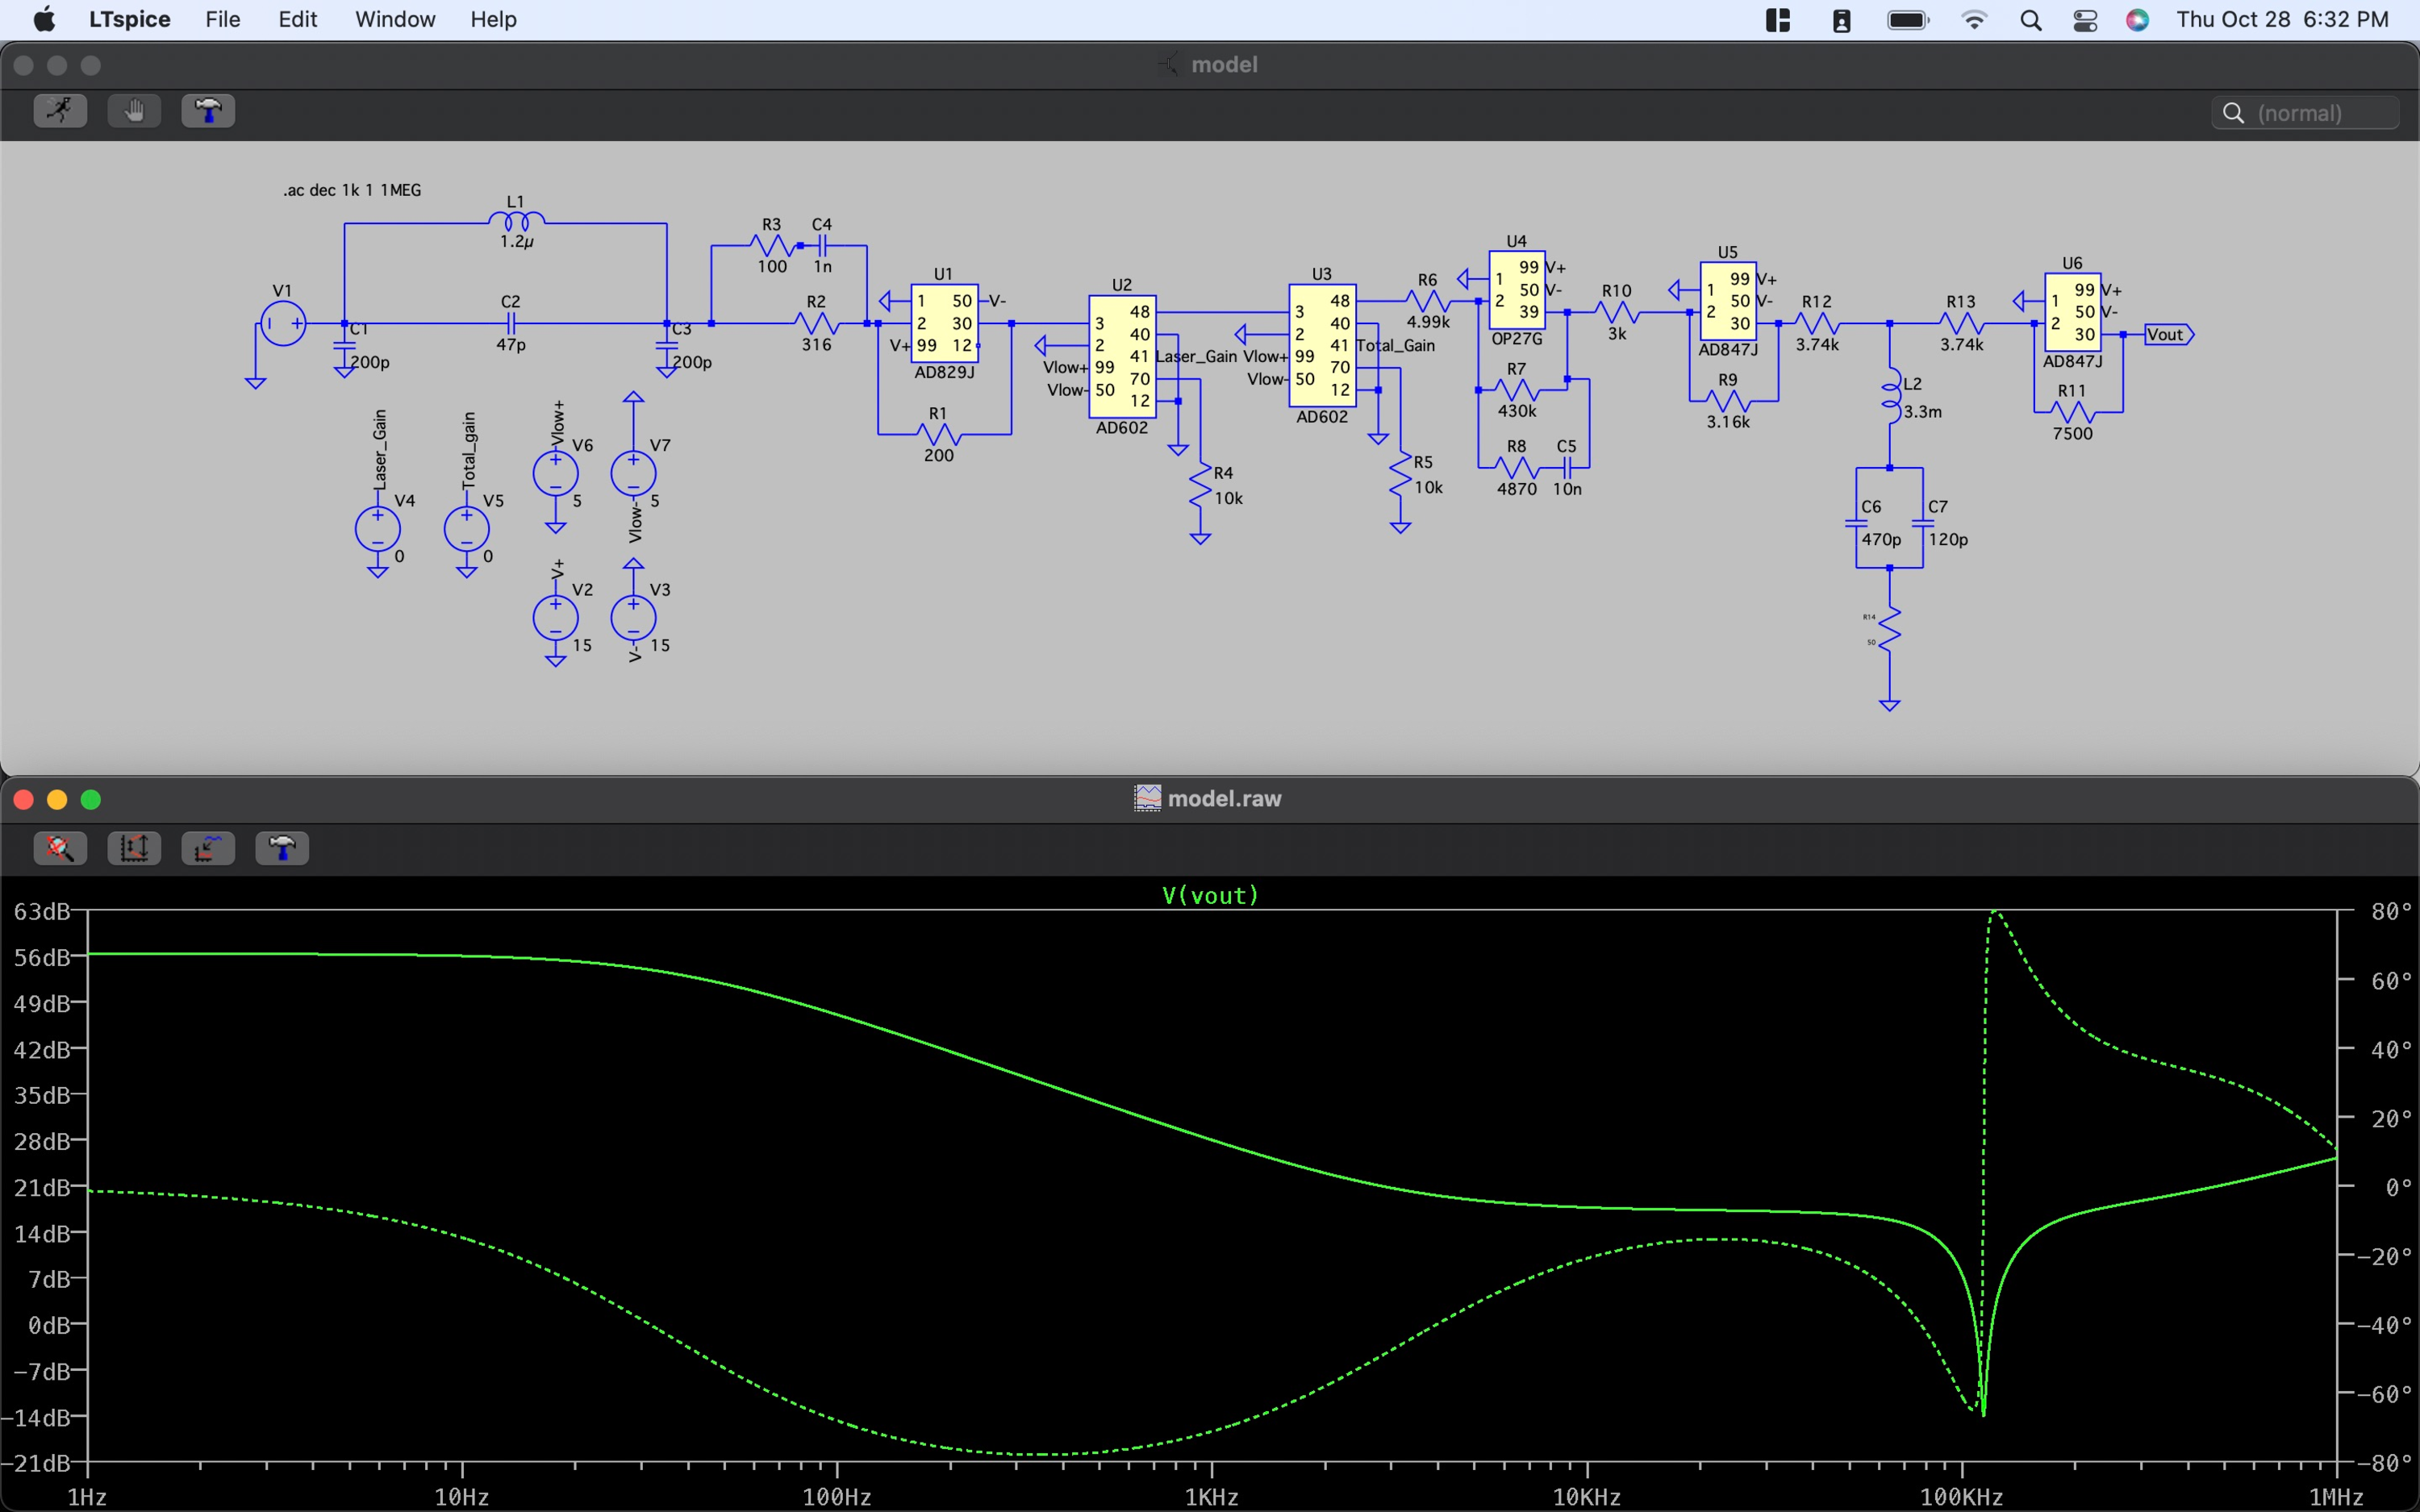
\includegraphics[width=\textwidth]{figs/ALGAAS/tfs/spice_FSS_tf.pdf}
    \caption{The FSS frequency response simulated in LTspice}
  \end{center}
  \label{fig:spiceFSS}
\end{figure}

\section{Measuring OLG [H]}

\begin{figure}[H]
  \begin{center}
    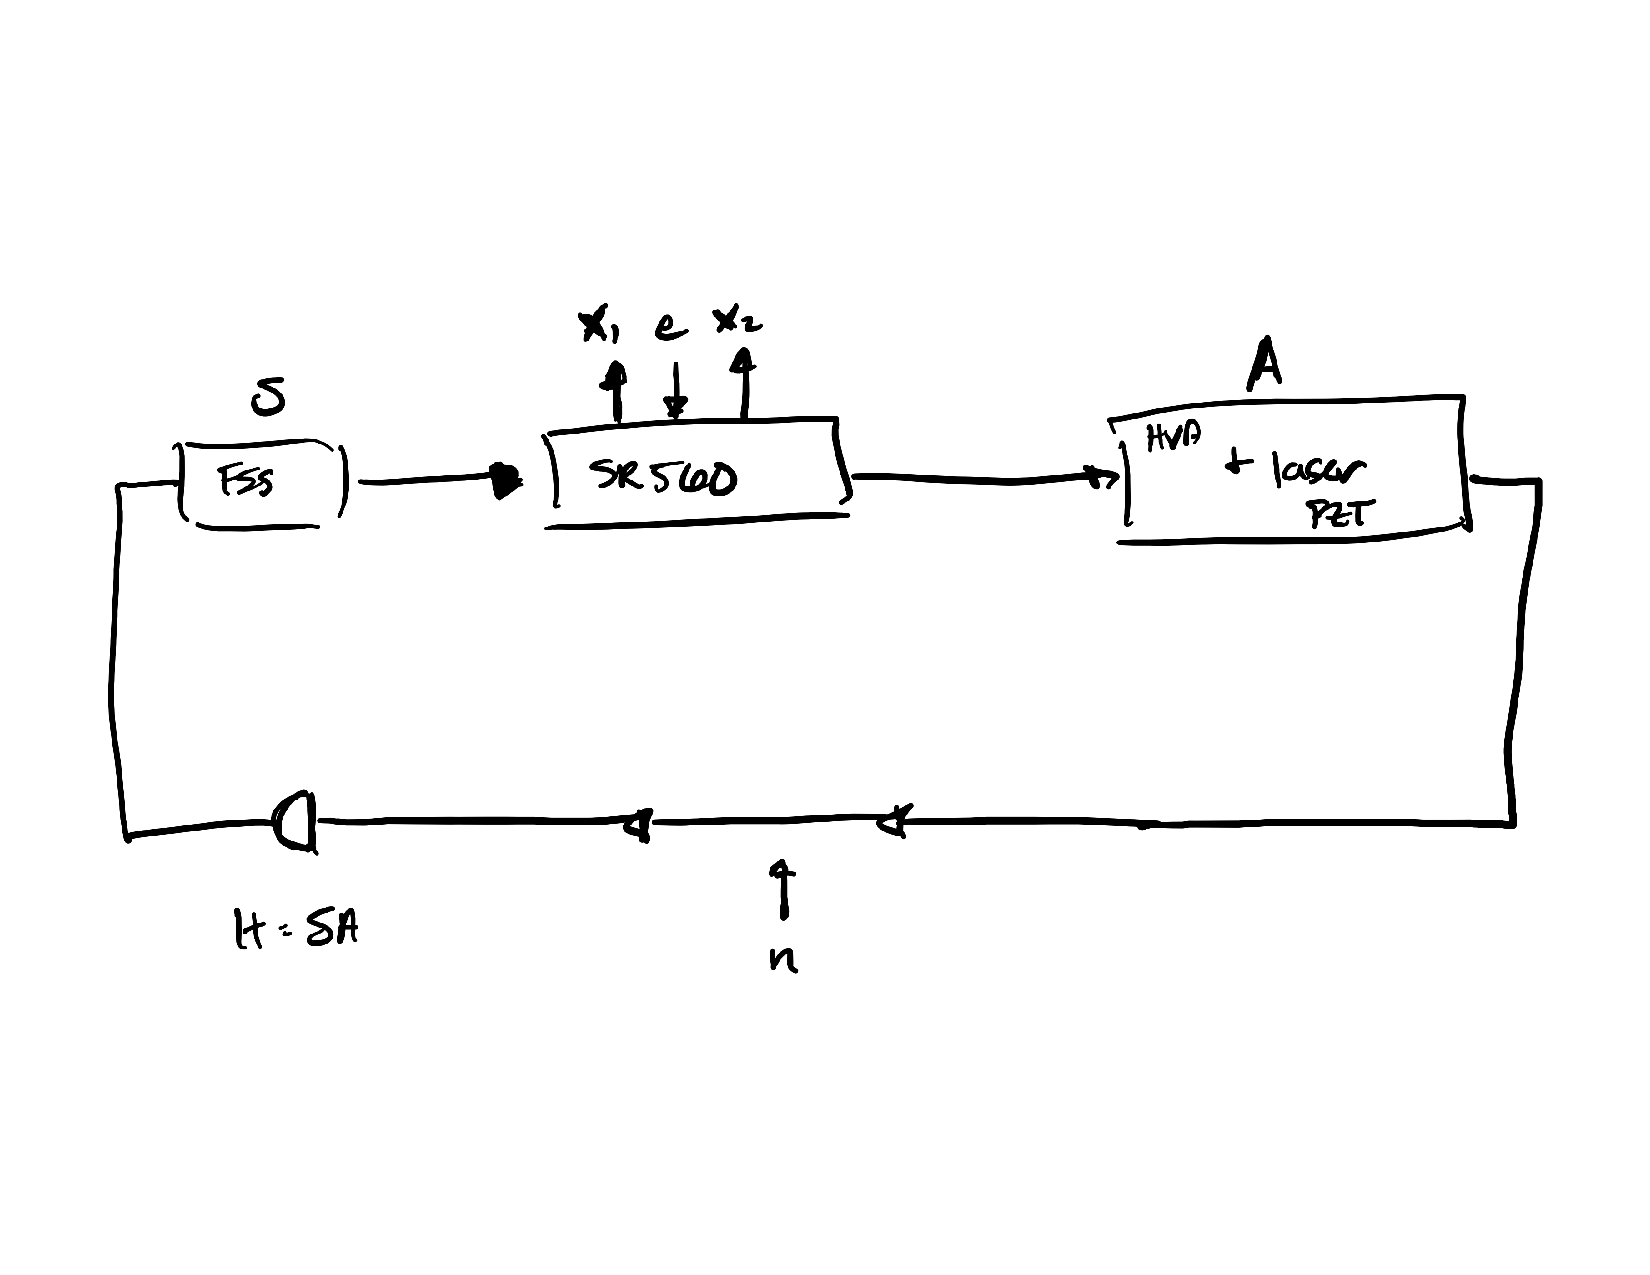
\includegraphics[width=.5\textwidth]{figs/ALGAAS/Loop_gain_measurement_drawn_diagram.pdf}
    \caption{Open loop gain measurement \textcolor{red}{drawn diagram}}
  \end{center}
  \label{fig:OLGmath}
\end{figure}

\textcolor{red}{x2 is the PSD taken immediately after the excitation point}
\begin{equation}
x_2 = e + He + H^2 e + \mathrm{H.O.T.s} = \frac{e + n}{1-H}
\end{equation}

\textcolor{red}{x1 is the PSD taken immediately prior to the excitation point}
\begin{equation}
x_1 = He + H^2e + H^3e + \mathrm{H.O.T.s}  = \frac{He}{1-H}
\end{equation}

We take the transfer function measurement $\zeta$:

\begin{equation}
\zeta = \frac{x_1}{x_2} = \frac{He/(1-H)}{(e+n)/(1-H)}
\end{equation}

Assuming the excitation is significantly larger than the noise ($e>>n$):

\begin{equation}
\zeta \approx H
\end{equation}
